\RequirePackage[l2tabu,orthodox]{nag}
\documentclass[a5paper,10pt,twoside,openany,article]{memoir}

%!TEX root = ../dissertation.tex
\usepackage{etoolbox}
\usepackage{pdflscape}
\usepackage{geometry}
\usepackage{xparse}

%% Various maths
\usepackage{amsthm,amsmath,amscd,amsfonts,amssymb,mathtools,amsthm}

%% Localization
\usepackage[main=russian,german,english]{babel}
\usepackage{fontspec}
\usepackage{iflang}


%% Fonts
\setmonofont{Courier New}
\defaultfontfeatures{Ligatures=TeX}
\setmainfont{Times New Roman}
\setsansfont{Arial}

%% Page geometry
\geometry{a5paper, top=14mm, bottom=14mm, inner=18mm, outer=10mm, footskip=5mm, nomarginpar}
\setlength{\topskip}{0pt}
\setlength{\footskip}{12.3pt}
\SingleSpacing

\makeevenhead{plain}{}{\thepage}{}
\makeoddhead{plain}{}{\thepage}{}
\makeevenfoot{plain}{}{}{}
\makeoddfoot{plain}{}{}{}
\pagestyle{plain}

%% Penalties
\tolerance=1414
\hbadness=1414
\emergencystretch=1.5em
\hfuzz=0.3pt
\vfuzz=\hfuzz
\clubpenalty=10000
\widowpenalty=10000
\brokenpenalty=4991

%% Tuning of Table of Contents
\renewcommand{\cftchapterdotsep}{\cftdotsep}
\setrmarg{2.55em plus1fil}
\renewcommand{\cftchapterpagefont}{\normalfont}
\renewcommand{\cftchapterleader}{\cftdotfill{\cftchapterdotsep}}
\renewcommand{\cftchapteraftersnum}{.\space}
\AtBeginDocument{\setsecnumformat{\csname the#1\endcsname\quad}}
\renewcommand*{\cftappendixname}{\appendixname\space}

%% Tuning of List of Figures/Tables
\makeatletter
\renewcommand{\@tocrmarg}{4em}
\renewcommand{\@pnumwidth}{3em}
\makeatother

%% Fonts and intervals of the basic things
\newcommand{\basegostsectionfont}{\fontsize{10pt}{12pt}\selectfont\bfseries}
\newlength{\gostindent}
\setlength{\gostindent}{30pt}
\setbeforesecskip{\gostindent}
\setaftersecskip{\gostindent}
\setbeforesubsecskip{\gostindent}
\setaftersubsecskip{\gostindent}
\setbeforesubsubsecskip{\gostindent}
\setaftersubsubsecskip{\gostindent}

\makechapterstyle{thesisgost}{%
\chapterstyle{default}%
\setlength{\beforechapskip}{0pt}%
\setlength{\midchapskip}{0pt}%
\setlength{\afterchapskip}{\gostindent}%
\renewcommand*{\chapnamefont}{\basegostsectionfont}%
\renewcommand*{\chapnumfont}{\basegostsectionfont}%
\renewcommand*{\chaptitlefont}{\basegostsectionfont}%
\renewcommand*{\chapterheadstart}{}%
\renewcommand*{\afterchapternum}{\quad}%
\renewcommand*{\printchapternum}{\centering\chapnumfont\thechapter}%
\renewcommand*{\printchaptername}{}%
\renewcommand*{\printchapternonum}{\centering}}

\makeatletter
\makechapterstyle{thesisgostchapname}{%
    \chapterstyle{thesisgost}
    \renewcommand*{\printchapternum}{\chapnumfont\thechapter}
    \renewcommand*{\printchaptername}{\centering\chapnamefont\@chapapp} %
}
\makeatother

\chapterstyle{thesisgost}
\setsecheadstyle{\basegostsectionfont\centering}
\setsecindent{0pt}
\setsubsecheadstyle{\basegostsectionfont\centering}
\setsubsecindent{0pt}
\setsubsubsecheadstyle{\basegostsectionfont\centering}
\setsubsubsecindent{0pt}
\sethangfrom{\noindent #1}

\chapterstyle{thesisgostchapname}
\renewcommand*{\cftchaptername}{\chaptername\space}

%% Making all the counters global
\counterwithout{equation}{chapter}
\counterwithout{equation}{section}
\counterwithout{equation}{subsection}
\counterwithout{figure}{chapter}
\counterwithout{figure}{section}
\counterwithout{figure}{subsection}
\counterwithout{table}{chapter}
\counterwithout{table}{section}
\counterwithout{table}{subsection}

\AtBeginDocument{%
\regtotcounter{totalcount@figure}%
\regtotcounter{totalcount@table}%
\regtotcounter{TotPages}%
}

%% Some not yet used magic to form Russian messages about sizes and counts
%% http://www.linux.org.ru/forum/general/6993203#comment-6994589 (используется totcount)
\makeatletter
\def\formbytotal#1#2#3#4#5{%
    \newcount\@c
    \@c\totvalue{#1}\relax
    \newcount\@last
    \newcount\@pnul
    \@last\@c\relax
    \divide\@last 10
    \@pnul\@last\relax
    \divide\@pnul 10
    \multiply\@pnul-10
    \advance\@pnul\@last
    \multiply\@last-10
    \advance\@last\@c
    \total{#1}~#2%
    \ifnum\@pnul=1#5\else%
    \ifcase\@last#5\or#3\or#4\or#4\or#4\else#5\fi
    \fi
}
\makeatother

%% A special environment for locale-dependent commands
%% Usage: \newlocalizedcommand{\YourCommandName}{expansion in English}{expansion in Russian}
%%        \renewlocalizedcommand{\YourCommandName}{expansion in English}{expansion in Russian}
\newcommand{\newlocalizedcommand}[3]{\newcommand{#1}{\IfLanguageName{russian}{#3}{#2}}}
\newcommand{\renewlocalizedcommand}[3]{\renewcommand{#1}{\IfLanguageName{russian}{#3}{#2}}}

%% Theorems (localized) %%
\newlocalizedcommand{\definitionname}{Definition}{Определение}
\newlocalizedcommand{\corollaryname}{Corollary}{Следствие}
\newlocalizedcommand{\theoremname}{Theorem}{Утверждение}
\newlocalizedcommand{\lemmaname}{Lemma}{Лемма}

\theoremstyle{definition}
\newtheorem{definition}{\definitionname}
\newtheorem{theorem}{\theoremname}
\newtheorem{lemma}{\lemmaname}
\newtheorem{corollary}{\corollaryname}

%% Paragraph formatting %%
\usepackage{indentfirst}
\AtBeginDocument{\setlength{\parindent}{2.5em}}

%% Enumerations (partially localized) %%
\usepackage{enumitem}
\setlist{nosep,labelindent=\parindent,leftmargin=*}

\makeatletter
\def\asbukx#1{\expandafter\@asbukx\csname c@#1\endcsname}
\def\@asbukx#1{\ifcase#1\or a\or б\or в\or г\or д\or е\or ж\or и\or к\or л\or м\or н\or п\or р\or с\or т\or у\or ф\or х\or ц\or ш\or щ\or э\or ю\or я\fi}
\def\Asbukx#1{\expandafter\@Asbukx\csname c@#1\endcsname}
\def\@Asbukx#1{\ifcase#1\or А\or Б\or В\or Г\or Д\or Е\or Ж\or И\or К\or Л\or М\or Н\or П\or Р\or С\or Т\or У\or Ф\or Х\or Ц\or Ш\or Щ\or Э\or Ю\or Я\fi}
\AddEnumerateCounter{\Asbukx}{\@Asbukx}{М}
\AddEnumerateCounter{\asbukx}{\@asbukx}{м}
\makeatother

\renewcommand{\labelitemi}{\normalfont\bfseries{--}}
\renewcommand\labelenumii{\arabic{enumii})}
\renewcommand\theenumii{\arabic{enumii}}
\renewlocalizedcommand{\labelenumi}{\alph{enumi})}{\asbukx{enumi})}
\renewlocalizedcommand{\theenumi}{\alph{enumi}}{\asbukx{enumi}}


%% Tuning of how floats look like
% We use floatrow/caption instead of memoir's poorly-working built-ins
\let\newfloat\undefined
\usepackage{caption}
\usepackage{floatrow}
\usepackage{subcaption}

%% Babel uses its own way to control captions, adhere to it
\addto{\captionsenglish}{%
\renewcommand{\figurename}{Figure}%
\renewcommand{\contentsname}{Contents}%
%\renewcommand{\ALG@name}{Algorithm}
}
\addto{\captionsrussian}{%
\renewcommand{\figurename}{Рисунок}%
\renewcommand{\contentsname}{Содержание}%
%\makeatletter
%\renewcommand{\ALG@name}{Листинг}%
%\makeatother
\renewcommand{\algorithmname}{Листинг}%
}

\floatsetup[figure]{style=plain, capposition=bottom}
\captionsetup[figure]{
    labelsep=endash,
    singlelinecheck=false,
    labelfont={normalsize,md},
    justification=centering,
    position=bottom
}
\floatsetup[table]{style=plain, capposition=top}
\captionsetup[table]{
    labelsep=endash,
    singlelinecheck=false,
    labelfont={normalsize,md},
    justification=justified,
    position=top
}
\floatsetup[algorithm]{style=plain, capposition=top}
\captionsetup[algorithm]{
    labelsep=endash,
    singlelinecheck=false,
    labelfont={normalsize,md},
    justification=justified,
    position=top
}
%\floatsetup[lstlisting]{style=plain, capposition=top}
%\captionsetup[lstlisting]{
%    labelsep=endash,
%    singlelinecheck=false,
%    labelfont={normalsize,md},
%    justification=justified,
%    position=top
%}

%% Tuning of table-of-contents

\settocdepth{subsection}            % до какого уровня подразделов выносить в оглавление
\setsecnumdepth{subsection}         % до какого уровня нумеровать подразделы

%% Custom math fonts

\usepackage{mathrsfs}

%% Graphics

\usepackage[dvipsnames, table, hyperref, cmyk]{xcolor}
\usepackage{graphicx}
\usepackage{pgfplots}
\pgfplotsset{compat=newest} 

% Include articles
\usepackage[final]{pdfpages}

%% Tables %%
\usepackage{tabularx}
\usepackage{longtable}
\usepackage{multirow,makecell}
\usepackage{hhline}
\usepackage{adjustbox}

\newcommand{\specialcell}[2][c]{%
  \begin{tabular}[#1]{@{}c@{}}#2\end{tabular}}

%% Hyperref %%
\usepackage{hyperref}
\definecolor{linkcolor}{rgb}{0,0,0}
\definecolor{citecolor}{rgb}{0,0,0}
\definecolor{urlcolor}{rgb}{0,0,0}

% No hypersetup here, as it needs some information not available here

%% Algorithmic environments %%
%\usepackage[linesnumbered,lined,boxed,commentsnumbered]{algorithm2e}
\usepackage{algorithm}
%\usepackage{algorithmic}
\usepackage[noend]{algpseudocode}
%\usepackage{amsmath}, amsthm,amsfonts,amssymb,amscd}

\algrenewcommand\algorithmicrequire{\textbf{Input:}}
\algrenewcommand\algorithmicensure{\textbf{Output:}}
\algnewcommand\algorithmicto{\textbf{to}}
\algrenewtext{For}[3] {\algorithmicfor\ $#1 \gets #2$ \algorithmicto\ $#3$ \algorithmicdo}
\algnewcommand\Continue{\textbf{continue}}
\algnewcommand\AndL{\textbf{and} }
\algnewcommand\OrL{\textbf{or} }
\algnewcommand\True{\textbf{True}}
\algnewcommand\False{\textbf{False}}

%% Counters
\usepackage[figure,table]{totalcount}
\usepackage{totcount}
\usepackage{totpages}

%% Misc localization commands %%
\let\origle\le   \renewlocalizedcommand{\le}{\origle}{\leqslant}
\let\origleq\leq \renewlocalizedcommand{\leq}{\origleq}{\leqslant}
\let\origge\ge   \renewlocalizedcommand{\ge}{\origge}{\geqslant}
\let\origgeq\geq \renewlocalizedcommand{\geq}{\origgeq}{\geqslant}
\let\origtan\tan \renewlocalizedcommand{\tan}{\origtan}{\operatorname{tg}}
\let\origcot\cot \renewlocalizedcommand{\cot}{\origcot}{\operatorname{ctg}}
\let\origcsc\csc \renewlocalizedcommand{\csc}{\origcsc}{\operatorname{cosec}}
\let\origempty\emptyset \renewlocalizedcommand{\emptyset}{\origempty}{\varnothing}

%% Misc technical things %%
\newcommand{\resetfloatcounters}{%
\setcounter{figure}{0}%
\setcounter{table}{0}%
\setcounter{theorem}{0}%
\setcounter{lemma}{0}%
\setcounter{definition}{0}%
\setcounter{corollary}{0}%
\setcounter{footnote}{0}%
}

%% Bibliography packages and configuration

\usepackage{csquotes} % biblatex рекомендует его подключать. Пакет для оформления сложных блоков цитирования.

%%% Загрузка пакета с основными настройками %%%
\makeatletter
\usepackage[backend=biber, bibencoding=utf8, sorting=none, style=gost-numeric, language=autobib,
            autolang=other, defernumbers=true, sortcites=true, doi=false, isbn=false, movenames=false, maxnames=99]{biblatex}
\ltx@iffilelater{biblatex-gost.def}{2017/05/03}%
{%\toggletrue{bbx:gostbibliography}%
\renewcommand*{\revsdnamepunct}{\addcomma}}{}
\makeatother

\renewcommand*{\newblockpunct}{\addperiod\addnbspace---\space\bibsentence}

\DefineBibliographyStrings{english}{pages = {p\adddot}}

\DefineBibliographyExtras{russian}{%
  \protected\def\bibrangedash{--\penalty\value{abbrvpenalty}}% almost unbreakable dash
  \protected\def\bibdaterangesep{\bibrangedash}%тире для дат
}
\DefineBibliographyExtras{english}{%
  \protected\def\bibrangedash{--\penalty\value{abbrvpenalty}}% almost unbreakable dash
  \protected\def\bibdaterangesep{\bibrangedash}%тире для дат
}

%Set higher penalty for breaking in number, dates and pages ranges
\setcounter{abbrvpenalty}{10000} % default is \hyphenpenalty which is 12
%Set higher penalty for breaking in names
\setcounter{highnamepenalty}{10000} % If you prefer the traditional BibTeX behavior (no linebreaks at highnamepenalty breakpoints), set it to ‘infinite’ (10 000 or higher).
\setcounter{lownamepenalty}{10000}

%% An environment which rewrites \cite to be \footfullcite for citations not in the author's list
\makeatletter
\newtoggle{footnotized@value}\togglefalse{footnotized@value}

\DeclareDocumentCommand{\trickycite}{oom}{%
\filteredcite{#3}%
\IfNoValueTF{#2}{%
\IfNoValueTF{#1}{%
% no #1 no #2
\iftoggle{footnotized@value}{\unspace\footfullcite{#3}}{\oldcite{#3}}%
}{%
% yes #1 no #2
\iftoggle{footnotized@value}{\unspace\footfullcite[#1]{#3}}{\oldcite[#1]{#3}}%
}}{
% yes #1 yes #2
\iftoggle{footnotized@value}{\unspace\footfullcite[#1][#2]{#3}}{\oldcite[#1][#2]{#3}}%
}}%
\newenvironment{footnotizeexcept}[1]{\begingroup%
\DeclareCiteCommand{\filteredcite}{}{\ifkeyword{#1}{\global\togglefalse{footnotized@value}}{\global\toggletrue{footnotized@value}}}{}{}%
\let\oldcite\cite\let\cite\trickycite}{\let\cite\oldcite\endgroup}
\makeatother


%!TEX root = ../dissertation.tex

%%% This is a place to put all definitions needed for this particular thesis to work

% Various definitions depending on how the bibliography is done

\addbibresource{dissertation.bib}
\DeclareSourcemap{
    \maps{
        \map{
            \step[fieldsource=medium, match=\regexp{Электронный\s+ресурс}, final]
            \step[fieldset=media, fieldvalue=eresource]
        }
    }
}

% Definitions and includes related for the text

\DeclareRobustCommand{\todo}{\textcolor{black}}
\newcommand{\revise}[1]{\textcolor{red}{#1}}
\graphicspath{{img/}}

\newcommand{\hamm}[1]{\mathcal{H}(#1)}
\newcommand{\tobinary}[1]{\mathcal{B}(#1)}
\newcommand{\theop}{\mathcal{X}}

\DeclareMathOperator*{\argmin}{arg\,min}
\DeclareMathOperator*{\argmax}{arg\,max}

\pgfplotscreateplotcyclelist{myplotcycle}{%
black\\%1
red!80!black\\%2
violet!80!black\\%3
gray!80!black\\%4
orange\\%5
brown!80!black\\%6
cyan!80!black\\%
green!70!black\\%7
green\\%8
blue!60!black\\%9
teal\\%10
magenta!70!black\\%11
yellow!90!black\\%12
}

%!TEX root = ../dissertation.tex

\newcommand{\thesisSpecialtyNumber}{05.13.17}
\newlocalizedcommand{\thesisSpecialtyName}{Theoretical foundations of computer science}{Теоретические основы информатики}
\newlocalizedcommand{\thesisAuthorFull}{Zakirzyanov Ilya Timurovich}{Закирзянов Илья Тимурович}
\newlocalizedcommand{\thesisAuthorShort}{Zakirzyanov~I.~T.}{Закирзянов~И.~Т.}
\newlocalizedcommand{\thesisDegreeGenitive}{Doctor of Philosophy}{кандидата технических наук}
\newlocalizedcommand{\thesisTitle}
{Deterministic finite automata inference methods using space search pruning when solving Boolean satisfiability problem}
{Методы генерации детерминированных конечных автоматов с использованием сокращения пространства поиска при решении задачи выполнимости}

\newcommand{\thesisOrganizationEng}{ITMO University}
\newlocalizedcommand{\thesisOrganizationNominative}{\thesisOrganizationEng}{Университет ИТМО}
\newlocalizedcommand{\thesisOrganizationLocative}  {\thesisOrganizationEng}{Университете ИТМО}
\newlocalizedcommand{\thesisOrganizationGenitive}  {\thesisOrganizationEng}{Университета ИТМО}
\newlocalizedcommand{\thesisOrganizationShortGenitive}{ITMO University}{Университета~ИТМО}
\newlocalizedcommand{\thesisOrganizationLogo}{
\includegraphics[width=0.28\linewidth]{logo_en}}{
\includegraphics[width=0.35\linewidth]{logo}}

\newlocalizedcommand{\thesisInTheLibrary}{in the library of \thesisOrganizationGenitive}{в библиотеке \thesisOrganizationGenitive}
\newlocalizedcommand{\thesisLibraryAddress}{49 Kronversky pr., Saint Petersburg, Russia}{197101, Санкт-Петербург, Кронверкский пр., д.49}
\newcommand{\thesisURLAddress}{\url{***}}

\newcommand{\thesisYear}{2020}
\newlocalizedcommand{\thesisCity}{Saint Petersburg}{Санкт-Петербург}
\newlocalizedcommand{\defenceDateTime}{\revise{on DD.MM.YYYY at HH:MM}}{\revise{DD.MM.YYYY в HH:MM}}
\newlocalizedcommand{\defenceAddress}{\revise{address, room number}}{\revise{адрес, аудитория}}

\newcommand{\defenceCouncilNumber}{02.18.00}
\newlocalizedcommand{\defenceCouncilAddress}{49 Kronversky pr., Saint Petersburg, Russia, room \revise{XXX}}{197101, Санкт-Петербург, Кронверкский пр., д.49, аудитория \revise{XXX}}
\newlocalizedcommand{\defenceCouncilSecretaryFull}{Mouromtsev Dmitry Ilich}{Муромцев Дмитрий Ильич}
\newlocalizedcommand{\defenceCouncilSecretaryDegree}{Doctor of Philosophy}{канд. техн. наук}
\newcommand{\defenceCouncilSecretarySignature}{
\includegraphics[width=2cm]{secretary-signature.png}}

\newlocalizedcommand{\supervisorFull}{Ulyantsev Vladimir Igorevich}{Ульянцев Владимир Игоревич}
\newlocalizedcommand{\supervisorShort}{Ulyantsev~V.~I.}{Ульянцев~В.~И.}
\newlocalizedcommand{\supervisorDegree}{Doctor of Philosophy}{канд. техн. наук}

% \newlocalizedcommand{\opponents}
% {\textbf{Tulupyev Alexander L'vovich},\par
%  \revise{Doctor of Physical and Mathematical Sciences},\par
%  Professor of Informatics Department\par
%  Federal State Budgetary Educational Institution of\par 
%  Higher Professional Education \par 
%  "Saint-Petersburg State University"\par
%  \vspace{1ex}\par
%  \textbf{Pavel Bernard Brazdil},\par
%  Doctor of Philosophy,
%  Professor of Engineer Faculty, 
%  Senior Researcher of INESC TEC’s 
%  Laboratory of Artificial Intelligence and Decision Support,
%  University of Porto, Porto, Portugal
% }{\textbf{Тулупьев Александр Львович},\par
%  доктор физико-математических наук, \par
%  профессор кафедры информатики\par
%  федерального государственного бюджетного\par
%  образовательного учреждения высшего \par
%  профессионального образования\par
%  "Санкт-Петербургский государственный университет"\par
%  \vspace{1ex}\par
%  \textbf{Pavel Bernard Brazdil},\par
%  Doctor of Philosophy,
%  Professor of Engineer Faculty, 
%  Senior Researcher of INESC TEC’s 
%  Laboratory of Artificial Intelligence and Decision Support,
%  University of Porto, Porto, Portugal
% }

\newcommand{\nociteallauthorpublications}{\nocite{
zakirzyanov2015LATA,
zakirzyanov2017DataMode,
zakirzyanov2019LATA,
kachalsky2018ICMLA,
Ovsiannikova2018INDIN,
zakirzyanov2020Vestnik,
zakirzyanov-kmu15,
zakirzyanov-kmu16,
zakirzyanov-kmu17,
zakirzyanov-kmu18,
zakirzyanov-kmu20}}

% Bibliography filters. As of now, they somewhat depend on which publications the author has.

\defbibfilter{thesisVak}{\keyword{labauthor:zakirzyanov}\and\keyword{phd:zakirzyanov}\and\keyword{index:vak}}
\defbibfilter{thesisIndexed}{\keyword{labauthor:zakirzyanov}\and\keyword{phd:zakirzyanov}\and\not\keyword{index:vak}\and\(\keyword{index:wos}\or\keyword{index:scopus}\)}
\defbibfilter{thesisEtc}{\keyword{labauthor:zakirzyanov}\and\keyword{phd:zakirzyanov}\and\not\keyword{index:vak}\and\not\keyword{index:wos}\and\not\keyword{index:scopus}\and\not\keyword{phd:program}}
\defbibfilter{nonThesisVak}{\keyword{labauthor:zakirzyanov}\and\not\keyword{phd:zakirzyanov}\and\keyword{index:vak}}
\defbibfilter{nonThesisIndexed}{\keyword{labauthor:zakirzyanov}\and\not\keyword{phd:zakirzyanov}\and\not\keyword{index:vak}\and\(\keyword{index:wos}\or\keyword{index:scopus}\)}
\defbibfilter{nonThesisEtc}{\keyword{labauthor:zakirzyanov}\and\not\keyword{phd:zakirzyanov}\and\not\keyword{index:vak}\and\not\keyword{index:wos}\and\not\keyword{index:scopus}}
\defbibfilter{thesisPrograms}{\keyword{phd:program}\and\keyword{labauthor:zakirzyanov}\and\keyword{phd:zakirzyanov}}

\newlocalizedcommand{\textDissPubs}{Author's publications on the topic of the thesis}{Публикации автора по теме диссертации}
\newlocalizedcommand{\textOtherPubs}{Author's publications on other topics}{Публикации автора по другим темам}
\newlocalizedcommand{\textRangeIndexed}{Publications indexed in Web of Science or Scopus}{Публикации в зарубежных изданиях, индексируемых в базах цитирования Web of Science или Scopus}
\newlocalizedcommand{\textRangeVak}{Publications indexed in Russian journal included in the List of the Higher Attestation Commission}{Публикации в журналах из перечня ВАК}
\newlocalizedcommand{\textRangeEtc}{Other publications (in Russian)}{Прочие публикации}
\newlocalizedcommand{\textProgram}{Registered computer programs}{Свидетельства о государственной регистрации программ для ЭВМ}

\defbibheading{headingDissIndexed}{\clearpage\chapter*{\textDissPubs}\section*{\textRangeIndexed}}
\defbibheading{headingVak}{\section*{\textRangeVak}}
\defbibheading{headingEtc}{\section*{\textRangeEtc}}
\defbibheading{headingOtherIndexed}{\clearpage\chapter*{\textOtherPubs}\section*{\textRangeIndexed}}
\defbibheading{headingProgram}{\section*{\textProgram}}

\newcommand{\printauthorpublications}{%
\printbibliography[filter=thesisIndexed,heading=headingDissIndexed]%
\printbibliography[filter=thesisVak,heading=headingVak]%
\printbibliography[filter=thesisEtc,heading=headingEtc]%
\printbibliography[filter=nonThesisIndexed,heading=headingOtherIndexed]%
\printbibliography[filter=nonThesisVak,heading=headingVak]%
\printbibliography[filter=nonThesisEtc,heading=headingEtc]%
\printbibliography[filter=thesisPrograms,heading=headingProgram]%
}


%!TEX root = ../dissertation.tex
%% Common misc %%

\newlocalizedcommand{\textAsManuscript}{As a manuscript}{На правах рукописи}
\newlocalizedcommand{\textSpecialty}{Specialty}{Специальность}
\newlocalizedcommand{\textThesisFulfilsRequirementsOf}{A thesis submitted in fulfillment of the requirements for the degree of}{Диссертация на соискание учёной степени}
\newlocalizedcommand{\textSupervisorIs}{Scientific advisor:}{Научный руководитель:}
\newlocalizedcommand{\textSynopsis}{Synopsis}{Реферат}
\newlocalizedcommand{\textWorkDoneIn}{The research was carried out at}{Работа выполнена в}
\newlocalizedcommand{\textOpponentsAre}{Official opponents:}{Официальные оппоненты:}

%% Title page %%

\newcommand{\thetitlepage}{
\setcounter{page}{1}
\thispagestyle{empty}
% organization name
{\centering\thesisOrganizationNominative\par}
\vspace{0pt plus2fill}
% organization logo + permissions
\noindent\begin{tabularx}{\linewidth}{lXr}
\vspace{0pt}\thesisOrganizationLogo & & \textAsManuscript \\
\end{tabularx}\par
\vspace{0pt plus6fill}
% author
{\centering\large\thesisAuthorFull\par}
\vspace{0pt plus1fill}
% title + specialty
{\centering\textbf{\large\thesisTitle}\par
\vspace{0pt plus2fill}
\textSpecialty\ \thesisSpecialtyNumber~---\par
\thesisSpecialtyName\par
\vspace{0pt plus2fill}
\textThesisFulfilsRequirementsOf\par
\thesisDegreeGenitive\par}
\vspace{0pt plus4fill}
% supervisor
\begin{flushright}
\textSupervisorIs\par\supervisorDegree\par\supervisorFull
\end{flushright}
% place + date
\vspace{0pt plus4fill}
{\centering\thesisCity~--- \thesisYear\par}
\newpage
}

%% Synopsis heading misc %%

\newlocalizedcommand{\markupDissertationCouncilSignature}
{Scientific Secretary of the\par\thesisOrganizationShortGenitive\par Dissertation Council \defenceCouncilNumber,\par\defenceCouncilSecretaryDegree}
{Ученый секретарь\par диссертационного совета\par\thesisOrganizationShortGenitive\par\defenceCouncilNumber,\par\defenceCouncilSecretaryDegree}
\newlocalizedcommand{\markupDefenceWillBeAt}
{The defence will be held on \defenceDateTime~at the meeting of the \thesisOrganizationShortGenitive\ Dissertation Council \defenceCouncilNumber~at \defenceCouncilAddress.}
{Защита состоится \defenceDateTime~на~заседании диссертационного совета \thesisOrganizationShortGenitive\ \defenceCouncilNumber~по адресу: \defenceCouncilAddress.}
\newlocalizedcommand{\markupThesisAvailableAt}
{The thesis is available \thesisInTheLibrary, \thesisLibraryAddress, and on the Web at \thesisURLAddress.}
{С диссертацией можно ознакомиться \thesisInTheLibrary\ по адресу: \thesisLibraryAddress, а также на сайте \thesisURLAddress.}

%% Synopsis %%

\newcommand{\labelsyn}[1]{\label{#1}}
\newcommand{\thesynopsis}[4]{
\begin{otherlanguage}{#1}
\setcounter{page}{1}
\begingroup
\let\extref\ref%
\renewcommand*{\thepage}{#2.\arabic{page}}
\renewcommand*{\thefigure}{#2.\arabic{figure}}
\renewcommand*{\thetable}{#2.\arabic{table}}
\renewcommand*{\ref}[1]{\extref{syn:#2:##1}}%
\renewcommand*{\labelsyn}[1]{\label{syn:#2:##1}}%
\begin{footnotizeexcept}{#3}
\begin{refsection}
\resetfloatcounters
{\centering\Large\textbf{\textSynopsis}\addcontentsline{toc}{chapter}{\textSynopsis}\par}
\input{#4}
\nociteallauthorpublications
\urlstyle{rm}\printauthorpublications\urlstyle{tt}
\newpage
\end{refsection}
\end{footnotizeexcept}
\endgroup
\end{otherlanguage}}

%!TEX root = ../dissertation.tex
%% Some constants for hypersetup were not known until user data is defined

\hypersetup{
    unicode,
    linktocpage=true,
    plainpages=false,
    colorlinks,
    linkcolor={linkcolor},
    citecolor={citecolor},
    urlcolor={urlcolor},
    pdftitle={\thesisTitle},
    pdfauthor={\thesisAuthorShort},
    pdfsubject={\thesisSpecialtyNumber\ \thesisSpecialtyName},
    pdfkeywords={},
    pdflang={en}
}


% \OnehalfSpacing*
% \setSpacing{1.42}
\linespread{1.42}

\begin{document}

% Обрезка титульников
\begin{otherlanguage}{russian}\thetitlepage\end{otherlanguage}
\begin{otherlanguage}{english}\thetitlepage\end{otherlanguage}

%Оглавление
\ifoddpage\null\else\newpage\thispagestyle{empty}\null\newpage\fi
\clearpage\tableofcontents*\newpage
\newcounter{savedpage}
\addtocounter{savedpage}{\value{page}}

% Рефераты на русском и английском языках
\thesynopsis{russian}{Р}{labauthor:zakirzyanov}{Synopsis/content-ru}
\thesynopsis{english}{S}{labauthor:zakirzyanov}{Synopsis/content-en}

% Основной текст диссертации
\setcounter{page}{\value{savedpage}}
\resetfloatcounters

% %!TEX root = ../dissertation.tex

\chapter*{Введение}                         % Заголовок
\addcontentsline{toc}{chapter}{Введение}    % Добавляем его в оглавление

%!TEX root = ../dissertation.tex
\textbf{Актуальность темы.} 

\textbf{Степень разработанности темы.}

\textbf{Целью} исследования является разработка точных методов генерации детерминированных конечных автоматов по имеющимся примерам поведения с использованием сокращения пространства поиска при решении задачи выполнимости.

Для~достижения указанной цели определены следующие \textbf{задачи}:
\begin{enumerate}
  \item Разработать точный метод построения ДКА по имеющимся примерам поведения с использованием <<компактных>> предикатов нарушения симметрии на основе алгоритма обхода графа в ширину.
  \item Разработать методы сокращения пространства поиска при решении задачи выполнимости для 
  построения ДКА по имеющимся примерам поведения, основанные на структурных особенностях искомого автомата.
  \item Разработать точный метод построения всех возможных ДКА по имеющимся примерам поведения с использованием программных средств решения задачи выполнимости.
  \item Разработать комбинированный точный метод построения ДКА по имеющимся примерам поведения на основе сведения к задаче выполнимости и с использованием подхода уточнения абстракции по контрпримерам.
  \item Разработать программный комплекс, реализующий все вышеуказанные методы.
  \item Провести экспериментальные исследования для оценки применимости и времени работы разработанных и реализованных методов, изложенных выше. 
\end{enumerate}

\textbf{Объект исследования}~{---} методы генерации конечных автоматных моделей.

\textbf{Предмет исследования}~{---} точные методы генерации детерминированных конечных автоматов по имеющимся примерам поведения.

\textbf{Соответствие паспорту специальности.} Данная диссертация соответствует пункту 5 <<\textbf{Разработка и исследование моделей и алгоритмов анализа данных, обнаружения закономерностей в данных и их извлечениях разработка и исследование методов и алгоритмов анализа текста}, устной речи и изображений.>>.

\emph{??? пункт 10 <<\textbf{Разработка основ} математической теории языков и грамматик, \textbf{теории конечных автоматов} и теории графов.>>}

\emph{??? пункт 7 <<\textbf{Разработка методов} распознавания образов, фильтрации, \textbf{распознавания и синтеза} изображений, \textbf{решающих правил}. Моделирование формирования эмпирического знания.>>}

\emph{??? пункт 3 <<Исследование методов и разработка средств кодирования информации в виде данных. Принципы создания языков описания данных, языков манипулирования данными, языков запросов. \textbf{Разработка и исследование моделей данных и новых принципов их проектирования}>>.}

\textbf{Основные положения, выносимые на~защиту:}
\begin{enumerate}
  \item Разработан точный метод построения ДКА по имеющимся примерам поведения с использованием <<компактных>> предикатов нарушения симметрии на основе алгоритма обхода графа в ширину.
  \item Разработаны методы сокращения пространства поиска при решении задачи выполнимости для построения ДКА по имеющимся примерам поведения, основанные на структурных особенностях искомого автомата.
  \item Разработан точный метод построения всех возможных ДКА по имеющимся примерам поведения с использованием программных средств решения задачи выполнимости.
  \item Разработан комбинированный точный метод построения ДКА по имеющимся примерам поведения на основе сведения к задаче выполнимости и с использованием подхода уточнения абстракции по контрпримерам.
\end{enumerate}

\textbf{Научная новизна} заключается в~следующем:
\begin{enumerate}
  \item Впервые точный метод построения ДКА по имеющимся примерам поведения с использованием предикатов нарушения симметрии на основе алгоритма обхода графа в ширину был предложен научным руководителем В.И.~Ульянцевым при участии автора диссертации.
  Новизна предложенного в данной работе метода заключается в использовании <<компактных>> предикатов нарушения симметрии --- пропозициональное кодирование данных предикатов на языке задачи выполнимости содержит квадратичное относительно размера автомата количество дизъюнктов вместо кубического из оригинального метода.
  Разработанный метод помимо уменьшения размера булевой формулы обеспечивает статистически значимое преимущество скорости работы по сравнению с существующими точными методами.
  \item Впервые были предложены методы сокращения пространства поиска при решении задачи выполнимости для построения ДКА по имеющимся примерам поведения, основанные на структурных особенностях искомого автомата.
  Использование данных методов обеспечивает статистически значимое преимущество скорости работы по сравнению с существующими точными методами. 
  \item Впервые был предложен точный метод построения всех возможных ДКА по имеющимся примерам поведения с использованием программных средств решения задачи выполнимости.
  Новизна предложенного метода заключается в использовании предикатов нарушения симметрии на основе алгоритма обхода графа в ширину, что позволяет оставить для рассмотрения единственного представителя для каждого класса эквивалентности по изоморфизму.
  \item Впервые был предложен комбинированный точный метод построения ДКА по имеющимся примерам поведения на основе сведения к задаче выполнимости и с использованием подхода уточнения абстракции по контрпримерам.
  Новизна предложенного метода заключается в использовании только части имеющихся примеров поведения при построении ДКА, что обеспечивает статистически значимое преимущество скорости работы по сравнению с существующими точными методами в случаях, когда число имеющихся примеров поведения излишне велико относительно размера искомого автомата.
\end{enumerate}

\textbf{Методология и методы исследования.} В работе используются методы теории автоматов, теории сложности, дискретной математики, объектно-ориентированное программирование, методы проведения и анализа экспериментальных исследований

\textbf{Достоверность} полученных результатов, подтверждается корректным обоснованием постановок задач, точной формулировкой критериев, а также результатами проведенных экспериментальных исследований по использованию предложенных в диссертации методов.

\textbf{Теоретическая значимость работы} состоит в том, что для задачи генерации ДКА по имеющимся примерам поведения было предложено пропозициональное кодирование предикатов нарушения симметрии на основе алгоритма обхода графа в ширину, содержащее асимптотически меньшее количество дизъюнктов.
Также для задачи генерации ДКА по имеющимся примерам поведения были предложены методы по сокращению пространства поиска при решении задачи выполнимости.
Помимо этого, был предложен метод для решения задачи построения всех различных неизоморфных ДКА по имеющимся примерам поведения, для решения которой ранее эффективных методов не существовало.
Также был предложен метод, объединяющий в себе два различных подхода: сведение к задаче выполнимости и уточнение абстракции по контрпримерам.

\textbf{Практическая значимость работы} состоит в том, что разработанные методы и реализованные в рамках программного комплекса на основе данных методов алгоритмы  позволяют ускорить и улучшить генерацию ДКА по имеющимся примерам поведения, что позволяет решать задачи более высокой сложности, выраженной в размере искомого автомата, в размере алфавита, в недостаточном или избыточном покрытии автомата примерами поведения.

\textbf{Участие в научно-исследовательских работах.} 
Результаты диссертации использовались при проведении НИР <<Разработка эффективных методов машинного обучения для построения детерминированных конечных автоматов на основе решения задачи выполнимости>> (грант РФФИ <<Мой первый грант>> 18-37-00425, 2018--2020 гг.) под руководством автора диссертации.

Полученные результаты также использовались при проведении следующих НИР:
\begin{itemize}
  \item <<Биоинформатика, машинное обучение, технологии программирования, теория кодирования, проактивные системы>> (субсидия \mbox{074-U01} в рамках государственной финансовой поддержки ведущих университетов Российской Федерации, 2013--2017 гг.);
  \item <<Методы, модели и технологии искусственного интеллекта в биоинформатике, социальных медиа, киберфизических, биометрических и речевых системах>>, (субсидия \mbox{08-08} в рамках государственной финансовой поддержки ведущих университетов Российской Федерации, 2018--2020 гг.).
\end{itemize}

\textbf{Апробация результатов работы.}
Основные результаты работы докладывались на следующих конференциях и семинарах:
\begin{enumerate}
  \item 9\textsuperscript{th} International Conference on Language and Automata Theory and Applications (LATA 2015). 2015, Ницца, Франция.
  \item 6\textsuperscript{th} International Symposium ``From Data to Models and Back (DataMod)''. 2017, Тренто, Италия.
  \item 13\textsuperscript{th} International Conference on Language and Automata Theory and Applications (LATA 2019). 2015, Санкт-Петербург.
  \item IV-VII Всероссийский Конгресс молодых ученых. 2015-2018, Санкт-Петербург.
  \item IX Конгресс молодых ученых. 2020, Санкт-Петербург.
  \item XLVI Научная и учебно-методическая Конференция Университета \mbox{ИТМО}. 2017, Санкт-Петербург.
  \item XLVIII Научная и учебно-методическая Конференция Университета ИТМО. 2019, Санкт-Петербург.
\end{enumerate}

\textbf{Личный вклад автора.}.
  Идея точного метода построения ДКА по имеющимся примерам поведения с использованием <<компактных>> предикатов нарушения симметрии на основе алгоритма обхода графа в ширину принадлежит совместно автору диссертации и Ж.~Маркешу-Сильве, реализация алгоритма на базе предложенного метода принадлежит лично автору диссертации, проведение вычислительных экспериментов принадлежит совместно автору диссертации и А.И.~Игнатьеву.
  Идея методов сокращения пространства поиска при решении задачи выполнимости для построения ДКА по имеющимся примерам поведения, основанные на структурных особенностях искомого автомата принадлежит совместно автору диссертации и Ж.~Маркешу-Сильве, реализация алгоритмов на базе предложенных методов принадлежит лично автору диссертации, проведение вычислительных экспериментов принадлежит совместно автору диссертации и А.И.~Игнатьеву.
  Идея точного метода построения всех возможных ДКА по имеющимся примерам поведения с использованием программных средств решения задачи выполнимости принадлежит совместно автору диссертации и научному руководителю В.И.~Ульянцеву, реализация алгоритма на базе предложенного метода и проведение вычислительных экспериментов принадлежит лично автору.
  Идея комбинированного точного метода построения ДКА по имеющимся примерам поведения на основе сведения к задаче выполнимости и с использованием подхода уточнения абстракции по контрпримерам принадлежит совместно автору диссертации и научному руководителю В.И.~Ульянцеву, реализация алгоритма на базе предложенного метода и проведение вычислительных экспериментов принадлежит лично автору.

\textbf{Публикации.}
Основные результаты по теме диссертации изложены в девяти публикациях, из них три опубликованы в изданиях, индексируемых в базе цитирования Scopus, одна публикация издана в журнале, рекомендованном ВАК.
Также у автора диссертации имеются две публикации по другим темам, из которых одна связана с машинным обучением, другая с построением автоматных моделей для кибер-физических систем, обе опубликованы в изданиях, индексируемых в базе цитирования Scopus. % Характеристика работы по структуре во введении и в автореферате не отличается (ГОСТ Р 7.0.11, пункты 5.3.1 и 9.2.1), потому её загружаем из одного и того же внешнего файла, предварительно задав форму выделения некоторым параметрам    % Введение
%!TEX root = ../dissertation.tex

\chapter{Обзор предметной области} \label{ch:review}

\section{Детерминированные конечные автоматы} \label{sec:dfa-def}

\emph{Алфавитом} $\Sigma$ называется некоторое конечное непустое множество символов.
\emph{Размером алфавита} $\Sigma$ называется число его символов~{---} $L = \abs{\Sigma}$.
В данной диссертации в основном будет рассматривать бинарный алфавит $\Sigma = \mathbb{B} = \{0, 1\}$.
\emph{Словом} (\emph{строкой}, \emph{цепочкой}) $\omega$ называется конечная последовательность символов некоторого алфавита. 
\emph{Длиной слова} называется число символов в нем, обозначается как $\abs{\omega}$.
Множество слов длины $k$ над алфавитом $\Sigma$ обозначается как $\Sigma^{k}$.
\emph{Пустой строкой} называется слово, не содержащее ни одного символа.
Такая строка, обозначаемая как $\varepsilon$, имеет нулевую длиной и может рассматриваться как слово над любым алфавитом~{---} $\Sigma^{0}=\{\varepsilon\}$.
Множество всех возможных слов, составленных из символов некоторого алфавита $\Sigma$, является его замыканием:
$$\Sigma^{*} = \bigcup_{k=0}^{\infty}\Sigma^{k}.$$
Подмножество множества всех слов над алфавитом $\Sigma$ называется \emph{языком}~--- $\mathcal{L} \subset \Sigma^{*}$.

\emph{Детерминированным конечным автоматом} (ДКА) называется пятерка $\mathcal{D} = \left(D,\Sigma,\delta,d_{1},D^{+}\right)$, где $D$~{---} конечное множество состояний, $\Sigma$~{---} алфавит входных символов, $\delta:D \times \Sigma \rightarrow D$~{---} \emph{функция переходов}, $d_{1}$~{---} \emph{стартовое} (\emph{начальное}) состояние, $D^{+} \subset D$~{---} множество \emph{допускающих} (\emph{принимающих}) состояний. 
В неявном виде также задано множество \emph{недопускающих} (\emph{отвергающих}) состояний $D^{-} = D \setminus D^{+}$.

Индуктивно определим вспомогательную \emph{расширенную функцию переходов} $\hat{\delta}: D \times \Sigma^{*} \rightarrow D$:
\begin{enumerate}
  \item для любого состояния $d_{i}$ верно, что переход по пустой строке не осуществляется~{---} $\hat{\delta}\left(d_{i},\varepsilon\right) = d_{i}$;
  \item для любого состояния $d_{i}$ верно, что переход по строке $\pi = \pi'c$, где $\pi,\pi' \in \Sigma^{*}$, $c \in \Sigma$, может быть определен следующим образом $\hat{\delta}\left(d_{i}, \pi\right) = \delta\left(\hat{\delta}\left(d_{i}, \pi'\right), c\right)$.
\end{enumerate}
Говорят, что ДКА $\mathcal{D}$ \emph{допускает} (\emph{принимает}) слово $\omega$, если $\hat{\delta}\left(d_{1}, \omega\right) \in D^{+}$. 
Иначе, если $\hat{\delta}\left(d_{1}, \omega\right) \in D^{-}$, говорят, что ДКА $\mathcal{D}$ \emph{не допускает} (\emph{отвергает}) слово $\omega$. 
Множество всех слов, допускаемых автоматом $\mathcal{D}$: $\mathcal{L}\left(D\right) = \{\omega \mid \hat{\delta}\left(d_{1}, \omega \right)\}$, называется языком автомата $\mathcal{D}$.

%!TEX root = ../dissertation.tex

\chapter{Компактные предикаты нарушения симметрии} 
\label{sec:tight}

Кодирование свойства BFS пронумерованности автомата, описанное в разделе~\ref{sec:review:sym-breaking:bfs-based}, состоящее из $\mathcal{O}\left(M^{3} + M^{2} \times L^{2}\right)$ дизъюнктов, слабо применимо на практике для ДКА большого размера, то есть при большом $M$. 
В данной главе описывается как модифицировать предикаты нарушения симметрии, рассмотренные ранее, таким образом, что для их булевого кодирования понадобится только $\mathcal{O}\left(M^{2} \times L\right)$ дизъюнктов.

\inote{подумать о подразделах}

%----------------------------------------------------------------------------------------

\section{Ревизия существующего кодирования}
\label{sec:tight:review}

Повторно кратко приведем наборы дизъюнктов, с помощью которых кодируются предикатов нарушения симметрии на основе алгоритма BFS, приведенные в разделе~\ref{sec:review:sym-breaking:bfs-based}.

\begin{equation}
\label{eq:t-def}
  \bigwedge_{1 \leq i < j \leq M} \left(t_{i,j} \leftrightarrow y_{i,l_{1},j} \vee y_{i,l_{2},j} \vee \ldots \vee y_{i,l_{L},j} \right)
\end{equation}
%
\begin{equation}
\label{eq:p-def}
  \bigwedge_{1 \leq i < j \leq M} \left(p_{j,i} \leftrightarrow t_{i,j} \wedge \neg t_{i - 1,j} \wedge \neg t_{i - 2, j} \wedge \ldots \wedge \neg t_{1,j}\right)
\end{equation}
%
\begin{equation}
\label{eq:p-alo}
  \bigwedge_{2 \leq j \leq M} \left(p_{j,1} \vee p_{j,2} \vee \ldots \vee p_{j,j - 1}\right)
\end{equation}
%
\begin{equation}
\label{eq:p-order}
  \bigwedge_{1 \leq k < i < j \leq M} \left(p_{j,i} \rightarrow \neg p_{j + 1, k}\right)
\end{equation}
%
\begin{equation}
\label{eq:m-def}
  \bigwedge_{1 \leq i < j \leq M} \bigwedge_{1 \leq n \leq L} \left(m_{i,l_{n},j} \leftrightarrow y_{i,l_{n},j} \wedge \neg y_{i,l_{n - 1}, j} \wedge \neg y_{i,l_{n - 2}, j} \wedge \ldots \wedge \neg y_{i,l_{1},j} \right)
\end{equation}
%
\begin{equation}
\label{eq:m-order}
  \bigwedge_{1 \leq i < j \leq M} \bigwedge_{1 \leq k < n \leq L} \left(p_{j,i} \wedge p_{j + 1, i} \wedge m_{i,l_{n}, j} \rightarrow \neg m_{i, l_{k}, j + 1}\right)
\end{equation}

Изучив формулы, приведенные выше, можно заключить, что:
\begin{enumerate}
  \item формула~\eqref{eq:t-def} содержит $\mathcal{O}\left(M^{2} \times L\right)$ дизъюнктов;
  \item формула~\eqref{eq:p-def} содержит $\mathcal{O}\left(M^{3}\right)$ дизъюнктов;
  \item формула~\eqref{eq:p-alo} содержит $\mathcal{O}\left(M\right)$ дизъюнктов;
  \item формула~\eqref{eq:p-order} содержит $\mathcal{O}\left(M^{3}\right)$ дизъюнктов;
  \item формула~\eqref{eq:m-def} содержит $\mathcal{O}\left(M^{2} \times L^{2}\right)$ дизъюнктов;
  \item формула~\eqref{eq:m-order} содержит $\mathcal{O}\left(M^{2} \times L^{2}\right)$ дизъюнктов.
\end{enumerate}
%
Таким образом, будет предложено новое кодирование для свойств, ранее выраженных формулами~\eqref{eq:p-def}, \eqref{eq:p-alo}, \eqref{eq:m-def} и \eqref{eq:m-order}.

Прежде всего, заметим, что формула~\eqref{eq:p-alo} задает свойство, что у каждого состояния $d_{j}$ (кроме начального) автомата $\mathcal{D}$ существует как минимум один родитель в дереве BFS, при этом с меньшим номером.
Однако, надо заметить, что по определению в любом дереве у любой вершины кроме корня существует ровно один родитель.
Тогда, можно добавить ограничение, задающее свойство, что у каждого состояния $d_{j}$ (кроме начального) автомата $\mathcal{D}$ существует не более одного родителя в дереве BFS, при этом с меньшим номером.
В совокупности два данных ограничения зададут вышеупомянутое свойство об единственности родителя.
Заметим, что ограничение, задающее свойство, что не более чем одна из $M$ переменных истинна, может быть выражено через $\mathcal{O}\left(M^2\right)$ или $\mathcal{O}\left(M\times \log M\right)$ дизъюнктов, что укладывается в целевой размер формулы $\mathcal{O}\left(M^{2} \times L\right)$ дизъюнктов.
\inote{либо написать как закодировать прямо тут, либо сослаться на раздел, где про это напишу}.

Фактически, новое ограничение можно записать следующим образом.
\begin{equation}
\label{eq:p-sum-eq-one}
  \bigwedge_{1 < j \leq M} \sum_{i=1}^{j-1}p_{j,i}=1
\end{equation}

%----------------------------------------------------------------------------------------

\section{Определение родительских переменных}
\label{sec:tight:p-def}

Формула $$\bigwedge_{1 \leq i < j \leq M} \left(p_{j,i} \leftrightarrow t_{i,j} \wedge \neg t_{i - 1,j} \wedge \neg t_{i - 2, j} \wedge \ldots \wedge \neg t_{1,j}\right)$$ при преобразовании в КНФ выражается через $\mathcal{O}\left(M^{3}\right)$ дизъюнктов, так как обе переменные $i$ и $j$ имеют область допустимых значений размера $M$, а также правая часть формулы имеет длину $O\left(M\right)$.
Так как переменные $i$ и $j$ независимы,то, чтобы сократить количество дизъюнктов, нужно сократить правую часть формулы.
Для этого предлагается ввести новые булевы переменные $\{\mathit{ft}_{i,j}\}_{0 \leq i < j \leq M}$.
Переменная $\mathit{ft}_{i,j}$ истинна тогда и только тогда, когда все переменные $t_{k,j}$, где $1 \leq k \leq i$, ложны (\textbf{f}alse $\boldsymbol{t}$ variables~{---} ложные переменные $t$).
Иными словами, $\mathit{ft}_{i,j} \leftrightarrow \neg t_{i,j} \wedge \neg t_{i - 1, j} \wedge \ldots \neg t_{1,j}$. 
Для $i = 0$ в явном виде определим, что $\mathit{ft}_{0,j} = 1$ для любого $j$.
Стоит, однако, заметить, что определение переменных $\mathit{ft}_{i,j}$, приведенное выше, требует также $\mathcal{O}\left(M^3\right)$ дизъюнктов, что не решает изначальную проблему.

При этом, можно заметить, что значение переменной $\mathit{ft}_{i,j}$ зависит от значения всех переменных $\mathit{ft}_{k,j}$, где $k < i$. Тогда, можно определить переменные $\mathit{ft}_{i,j}$ рекурсивно:

\begin{equation}
\label{eq:ft-def}
  \mathit{ft}_{i,j} \leftrightarrow 
    \begin{cases} 
      1                               & i = 0, 1 \leq j \leq M \\
      \mathit{ft}_{i-1,j} \wedge \neg t_{i,j}  & 1 \leq i < j \leq M
    \end{cases} 
\end{equation}
%
При преобразовании в КНФ формула~\eqref{eq:ft-def} будет состоять из $\mathcal{O}\left(M^{2}\right)$ дизъюнктов.

Используя новые переменные $\mathit{ft}_{i,j}$ формулу~\eqref{eq:p-def} можно переписать следующим образом.
%
\begin{equation}
\label{eq:p-def-tight}
  \bigwedge_{1 \leq i < j \leq M} \left(p_{j,i} \leftrightarrow t_{i,j} \wedge \mathit{ft}_{i-1,j}\right)
\end{equation}
%
В данной формуле решена проблема длинной правой части и общее число дизъюнктов, требуемых для кодирования переменных $p_{j,i}$, также $\mathcal{O}\left(M^{2}\right)$. 

%----------------------------------------------------------------------------------------

\section{Порядок детей с помощью родительных переменных}
\label{sec:tight:p-order}

\inote{БЛЯ! Мы по поводу этого раздела много выясняли, спорили с Жуаном, как правильно тут все устроено и т.д. Потому что выглядит все реально сложно. И только сейчас я понял, что это можно сделать ровно также как в разделе~\ref{sec:tight:m-order}}
\inote{Переписать этот раздел}
\inote{И, вероятно, всю главу тогда можно единообразно переписать}

Формула $$\bigwedge_{1 \leq k < i < j \leq M} \left(p_{j,i} \rightarrow \neg p_{j + 1, k}\right)$$ при преобразовании в КНФ выражается через $\mathcal{O}\left(M^{3}\right)$ дизъюнктов, так как все три переменные $i$, $j$ и $k$ имеют домен размера $M$.
Переменные $i$ и $j$ являются независимыми, поэтому сократить размер всей формулы можно только избавившись от переменной $k$.

Фактически, данная формула задает ограничение, что родитель состояния $d_{j + 1}$ автомата $\mathcal{D}$ имеет номер не меньший, чем номер родителя состояния $d_{j}$. 
Также можно заметить, что учитывая ограничение, заданное формулой~\eqref{eq:p-sum-eq-one}, двоичное число $\mathbf{p_{j}}=\overline{p_{j,1}p_{j,2}\ldots p_{j,j-1}}$ состоит из $j - 2$ нулей и одной единицы.
Тогда рассматриваемая формула говорит, что в числе $\mathbf{p_{j + 1}}$ единственная единица стоит не левее чем в векторе $\mathbf{p_{j}}$ (и наоборот, что в числе $\mathbf{p_{j}}$ единственная единица стоит не правее чем в векторе $\mathbf{p_{j + 1}}$). 
Для удобства сравнения данных чисел, рассматривается расширенное число $\tilde{\mathbf{p_{j}}} = \overline{p_{j,1}p_{j,2}\ldots p_{j,j-1}0}$.
В контексте имеющейся формулы расширенное число не отличается от обычного, так как в нем все еще содержится ровно одна единица на том же месте, что и раньше (считая, слева), но теперь двоичные числа $\tilde{\mathbf{p_{j}}}$ и $\mathbf{p_{j+1}}$ имеют одинаковое число цифр.
Тогда исходная формула фактически задает ограничение $\tilde{\mathbf{p_{j}}} \geq \mathbf{p_{j + 1}}$.
С помощью $\mathbf{p_{j}}^{\mathbf{i}}$ далее в данном разделе будет обозначаться двоичное число, являющееся суффиксом числа $\mathbf{p_{j}}$, начинающимся с $i$-ой цифры и заканчивая последней: $\mathbf{p_{j}}^{\mathbf{i}}=\overline{p_{j,i}p_{j,i+1}\ldots p_{j,j - 1}}$.
Аналогично, $\tilde{\mathbf{p_{j}}}^{\mathbf{i}}=\overline{p_{j,i}p_{j,i+1}\ldots p_{j,j}}$.

Для сравнения необходимо ввести новые булевы переменные $\{\mathit{geq}_{j,i}\}_{1 < j \leq M, 1 \leq i \leq j + 1}$.
Переменная $\{\mathit{geq}_{j,i}\}$ истинна тогда и только тогда, когда число $\tilde{\mathbf{p_{j}}}^{\mathbf{i}}$ больше или равно (\textbf{g}reater or \textbf{eq}ual) чем число $\mathbf{p_{j + 1}}^{\mathbf{i}}$, а значит и единица во втором числе находится не левее чем в первом. 
Определить переменные $\mathit{geq}_{j,i}$ можно рекурсивно следующим образом:
%
\begin{equation}
\label{eq:geq-def}
  \mathit{geq}_{j,i} \leftrightarrow 
    \begin{cases} 
      1                               & i = j + 1, 1 \leq j \leq M \\
      \mathit{geq}_{j,i + 1} \wedge \left(p_{j,i} \leftrightarrow p_{j + 1, i}\right) \vee p_{j,i} \wedge \neg p_{j + 1, i}  & 1 \leq i \leq j \leq M
    \end{cases} 
\end{equation}

Ограничение $\mathit{geq}_{j,j + 1} = 1$ задает исходное значение для рекурсивного определения переменных $\mathit{geq}_{j,i}$.
Далее, число $\tilde{\mathbf{p_{j}}}^{\mathbf{i}}$ больше или равно числа $\mathbf{p_{j + 1}}^{\mathbf{i}}$, то есть $\mathit{geq}_{j,i} = 1$, если $i$-ый бит чисел $\tilde{\mathbf{p_{j}}}$ и $\mathbf{p_{j + 1}}$ совпадает, а для суффиксов $\tilde{\mathbf{p_{j}}}^{\mathbf{i + 1}}$ и $\mathbf{p_{j + 1}}^{\mathbf{i + 1}}$ верно, что первый больше либо равен второго, или если $i$-ый бит числа $\tilde{\mathbf{p_{j}}}$ равен единице, а числа $\mathbf{p_{j + 1}}$~{---} нулю.
Последнее верно, так как оба числа содержат по одной единице и вне зависимости от того, где находится единица во втором числе, правее или левее, число $\tilde{\mathbf{p_{j}}}^{\mathbf{i}}$ строго больше числа $\mathbf{p_{j + 1}}^{\mathbf{i}}$.

Для упрощения записи и уменьшения размера дизъюнктов можно ввести еще одни вспомогательные переменные $\{\mathit{peq}_{j,i}\}_{1 \leq i \leq j \leq M}$.
Переменная $\mathit{peq}_{j,i}$ истинна тогда и только тогда, когда $p_{j,i} = p_{j + 1,i}$.
%
\begin{equation}
\label{eq:peq-def}
  \mathit{peq}_{j,i} \leftrightarrow \left(p_{j,i} \leftrightarrow p_{j + 1, i}\right) 
\end{equation}


Тогда формула~\eqref{eq:geq-def} примет окончательный вид:
%
\begin{equation}
\label{eq:geq-def2}
  \mathit{geq}_{j,i} \leftrightarrow 
    \begin{cases} 
      1                               & i = j + 1, 1 \leq j \leq M \\
      \mathit{geq}_{j,i + 1} \wedge \mathit{peq}_{j,i} \vee p_{j,i} \wedge \neg p_{j + 1, i}  & 1 \leq i \leq j \leq M
    \end{cases} 
\end{equation}
%
При преобразовании в КНФ формула~\eqref{eq:geq-def2} будет состоять из $\mathcal{O}\left(M^{2}\right)$ дизъюнктов.

Используя новые переменные $\mathit{geq}_{i,j}$ формулу~\eqref{eq:p-order} можно переписать следующим образом.
%
\begin{equation}
\label{eq:p-order-tight}
  \bigwedge_{1 < j \leq M} \mathit{geq}_{j,1}
\end{equation}
%
Действительно, $\mathit{geq}_{j,1} = 1 \Leftrightarrow \tilde{\mathbf{p_{j}}} = \tilde{\mathbf{p_{j}}}^\mathbf{1} \geq \mathbf{p_{j + 1}}^{\mathbf{1}} = \mathbf{p_{j + 1}}$.

Таким образом, формула~\eqref{eq:p-def-tight} выражается через $\mathcal{O}\left(M\right)$ дизъюнктов, а формулы~\eqref{eq:peq-def} и~\eqref{eq:geq-def2}~{---} через $\mathcal{O}\left(M^{2}\right)$ дизъюнктов.

%----------------------------------------------------------------------------------------

\section{Определение переменных минимального символа}
\label{sec:tight:m-def}

Формула $$\bigwedge_{1 \leq i < j \leq M} \bigwedge_{1 \leq n \leq L} \left(m_{i,l_{n},j} \leftrightarrow y_{i,l_{n},j} \wedge \neg y_{i,l_{n - 1}, j} \wedge \neg y_{i,l_{n - 2}, j} \wedge \ldots \wedge \neg y_{i,l_{1},j} \right)$$ при преобразовании в КНФ выражается через $\mathcal{O}\left(M^{2} \times L^{2}\right)$ дизъюнктов, так как обе переменные $i$ и $j$ имеют область допустимых значений размера $M$, переменная $n$~{---} размера $L$, а также правая часть формулы имеет длину $O\left(L\right)$.
Так как переменные $i$, $j$ и $n$ независимы,то, чтобы сократить количество дизъюнктов, нужно сократить правую часть формулы.
Можно заметить, что данная формула по своей структуре аналогична той, что рассматривалась в разделе~\ref{sec:tight:p-def}.
Тогда аналогично можно ввести новые булевы переменные $\{\mathit{fy}_{i,l_{n},j}\}_{0 \leq i < j \leq M,0 \leq n \leq M}$.
Переменная $\mathit{fy}_{i,l_{n},j}$ истинна тогда и только тогда, когда все переменные $y_{i,l_{k},j}$, где $1 \leq k \leq n$, ложны (\textbf{f}alse $\boldsymbol{y}$ variables~{---} ложные переменные $y$).
Иными словами, $\mathit{fy}_{i,l_{n},j} \leftrightarrow \neg y_{i,l_{n},j} \wedge \neg y_{i, l_{n - 1}, j} \wedge \ldots \neg y_{i,l_{1},j}$. 
Для $n = 0$ в явном виде определим, что $\mathit{fy}_{i,l_{0},j} = 1$ для любых $i,j$.
Далее, аналогично тому, как это было сделано в разделе~\ref{sec:tight:p-def}, определим переменные $\mathit{fy}_{i,l_{n},j}$ рекурсивно.

\begin{equation}
\label{eq:fy-def}
  \mathit{fy}_{i,l_{n},j} \leftrightarrow 
    \begin{cases} 
      1                               & 1 \leq i < j \leq M, n = 0 \\
      \mathit{fy}_{i,l_{n - 1},j} \wedge \neg y_{i,l_{n},j}  & 1 \leq i < j \leq M, 1 \leq n \leq L
    \end{cases} 
\end{equation}
%
При преобразовании в КНФ формула~\eqref{eq:fy-def} будет состоять из $\mathcal{O}\left(M^{2} \times L\right)$ дизъюнктов.

Используя новые переменные $\mathit{fy}_{i,l_{n},j}$ формулу~\eqref{eq:m-def} можно переписать следующим образом.
%
\begin{equation}
\label{eq:m-def-tight}
  \bigwedge_{1 \leq i < j \leq M} \bigwedge_{1 \leq n \leq L} \left(m_{i,l_{n},j} \leftrightarrow y_{i,l_{n},j} \wedge \mathit{fy}_{i,l_{n - 1},j} \right)
\end{equation}
%
В данной формуле решена проблема длинной правой части и общее число дизъюнктов, требуемых для кодирования переменных $m_{i,l_{n},j}$, также $\mathcal{O}\left(M^{2} \times L\right)$. 

%----------------------------------------------------------------------------------------

\section{Порядок детей одного родителя}
\label{sec:tight:m-order}

Формула $$\bigwedge_{1 \leq i < j \leq M} \bigwedge_{1 \leq k < n \leq L} \left(p_{j,i} \wedge p_{j + 1, i} \wedge m_{i,l_{n}, j} \rightarrow \neg m_{i, l_{k}, j + 1}\right)$$ при преобразовании в КНФ выражается также через $\mathcal{O}\left(M^{2} \times L^{2}\right)$ дизъюнктов, так как обе переменные $i$ и $j$ имеют область допустимых значений размера $M$, а обе переменные $n$ и $k$~{---} размера $L$.
Переменные $i$,$j$ и $n$ являются независимыми, поэтому сократить размер всей формулы можно только избавившись от переменной $k$.
Можно заметить, что данная формула по своей структуре аналогична той, что рассматривалась в разделе~\ref{sec:tight:p-order}.
Тогда аналогично можно ввести новые булевы переменные $\{\mathit{fm}_{i,l_{n},j}\}_{0 \leq i < j \leq M,0 \leq n \leq M}$.
Переменная $\mathit{fm}_{i,l_{n},j}$ истинна тогда и только тогда, когда все переменные $m_{i,l_{k},j}$, где $1 \leq k \leq n$, ложны (\textbf{f}alse $\boldsymbol{m}$ variables~{---} ложные переменные $m$).
Иными словами, $\mathit{fm}_{i,l_{n},j} \leftrightarrow \neg m_{i,l_{n},j} \wedge \neg m_{i, l_{n - 1}, j} \wedge \ldots \neg m_{i,l_{1},j}$. 
Для $n = 0$ в явном виде определим, что $\mathit{fm}_{i,l_{0},j} = 1$ для любых $i,j$.
Далее, аналогично тому, как это было сделано в разделе~\ref{sec:tight:p-order}, определим переменные $\mathit{fm}_{i,l_{n},j}$ рекурсивно.

\begin{equation}
\label{eq:fm-def}
  \mathit{fm}_{i,l_{n},j} \leftrightarrow 
    \begin{cases} 
      1                               & 1 \leq i < j \leq M, n = 0 \\
      \mathit{fm}_{i,l_{n - 1},j} \wedge \neg m_{i,l_{n},j}  & 1 \leq i < j \leq M, 1 \leq n \leq L
    \end{cases} 
\end{equation}
%
При преобразовании в КНФ формула~\eqref{eq:fm-def} будет состоять из $\mathcal{O}\left(M^{2} \times L\right)$ дизъюнктов.

Используя новые переменные $\mathit{fm}_{i,l_{n},j}$ формулу~\eqref{eq:m-order} можно переписать следующим образом.
%
\begin{equation}
\label{eq:m-order-tight}
  \bigwedge_{1 \leq i < j < M} \bigwedge_{1 \leq n \leq L} \left(p_{j,i} \wedge p_{j + 1, i} \wedge m_{i,l_{n}, j} \rightarrow \neg \mathit{fm}_{i, l_{n - 1}, j + 1}\right)
\end{equation}
%
Таким образом общее число дизъюнктов, требуемых для ограничения порядка детей одного состояния, равняется $\mathcal{O}\left(M^{2} \times L\right)$. 

%!TEX root = ../dissertation.tex

\chapter{Подходы к сокращению пространства поиска, основанные на структурных особенностях автомата} 
\label{sec:pruning}

В данной главе предлагаются новые методы по сокращению пространства поиска в задаче генерации ДКА минимального размера по заданным словарям. 
Данные методы не являются необходимыми для нахождения соответствующего автомата, но помогают сделать это быстрее.
В основе предлагаемых методов лежит использование структурных особенностей BFS пронумерованного ДКА, а также связь между расширенным префиксным деревом и ДКА.

\section{Полное дерево обхода в ширину}
\label{sec:pruning:bfs-tree}

\inote{рисунок дерева}

На рисунке \inote{ссылка} показано полное BFS дерево, построенное по некоторому автомату.
Данное дерево является полным, так как у каждой его внутренней вершины имеется по $L$ детей.
Тогда данное дерево показывает максимально возможные номера, которые могут быть у детей некоторого состояния $d_{i}$.
Действительно, нельзя добавить в данное дерево новые вершины, которые будут иметь номер между $i$ и $i \cdot L + 1$, так как все возможные позиции заняты.
В то же время, если удалить какие-то из вершин правее или ниже вершины $d_{i}$, то номера детей могут только уменьшиться.
Далее будут представлены дополнительные ограничения, которые следуют из рисунка \inote{ссылка}.

\paragraph{Сокращение области определения родительских переменных.}
У некоторого состояния $d_{i}$, где $1 \leq i < M$, детьми в BFS дереве могут быть только состояния с номерами от $i + 1$ до $\min\left(i \cdot L + 1, M\right)$.
Так как в BFS дереве номер ребенка всегда больше номера родителя, то нижняя граница тривиальна.
Рисунок \inote{ссылка} иллюстрирует обоснование верхней границы.
Действительно, можно доказать по индукции, что состояния на $k$-ом уровне имеют номера от $\sum_{r = 0}^{k - 1}L^{r} + 1$ до $\sum_{r = 0}^{k}L^{r}$.
База индукции при $k = 0$, очевидно, верна.
Если для некоторого слоя $k$ утверждение выше верно, то для слоя $k + 1$ верно, что нумерация состояний на нем начинается с $\sum_{r = 0}^{k - 1}L^{r} + 1$, а всего вершин $\left(\sum_{r = 0}^{k}L^{r} - \left(\sum_{r = 0}^{k - 1}L^{r} + 1\right) + 1\right) \cdot L = L^{k} * L = L^{k + 1}$, из чего следует, что последнее состояние имеет номер $\sum_{r = 0}^{k}L^{r} + L^{k + 1} = \sum_{r = 0}^{k + 1}L^{r}$.

\inote{возможно, оформить в виде полноценной теоремы и доказательства.}

Выразить данное свойство можно, либо определив переменные для соответствующей области определения~{---} $\{p_{j,i}\}_{1 \leq i < j \leq min(i \cdot L + 1, M)}$, либо в явном виде указав, что $p_{j,i} = 0$ при $j > i \cdot L + 1$.

\paragraph{Сокращение области определения переменных перехода и переменных наличия переходов.}
Помимо закономерностей между номерами родителей и детей в BFS пронумерованном автомате, можно заметить более общую закономерность относительно переходов.
Из состояния $d_{i}$ в BFS пронумерованном автомате не может в принципе существовать перехода в состояние $d_{j}$ если $j > i \cdot L + 1$.
Действительно, из доказанного в предыдущей секции следует, что у состояния $d_{j}$ родителем должно быть состояние $d_{k}$, где $k > i$.
Но, если существует из состояния $d_{i}$ существует переход в состояние $d_{j}$, то по принципу BFS обхода родителем состояния $d_{j}$ должно быть состояние $d_{k}$, где $k \leq i$.
Получившееся противоречие доказывает исходное утверждение.
Таким образом, можно сделать заключение, что $y_{i,l,j} = 0$ при $j > i \cdot L + 1; l \in \Sigma$.

Как следствие, по определению переменных наличия переходов верно, что $t_{i, j} = 0$ при $j > i \cdot L + 1$.

\inote{$y_{i,l,iL+2-j}$ --- пока скипнул, может добавить про них}

%----------------------------------------------------------------------------------------

\section{Свойство непрерывности родительских переменных}
\label{sec:pruning:continuity}

Помимо того, что у каждого состояния $d_{i}$ автомата $\mathcal{D}$ детьми могут быть состояния с номерами от $i + 1$ до $i \cdot L + 1$, можно утверждать, что состояние $d_{i}$ может быть родителем не более чем $L$ состояний, которые при этом пронумерованны последовательно.
Количество детей ограничено размером алфавита, так как рассматриваемый автомат является детерминированным.
Последовательная нумерация следует из структуры алгоритма BFS~{---} дети некоторого состояния поочередно добавляются в очередь и им присваиваются последовательные номера.
Данное свойство можно назвать \emph{свойством непрерывности}.
Для булевого кодирования предикатов нарушения симметрии данное свойство означает, что для фиксированного $i$ переменные $p_{j,i}$ ложны для всех $j$, кроме некоторого отрезка $[j_{0},\ldots,j_{s}]$, где $1 \leq j_{0} \leq j_{s} \leq M, s\leq L$.

Можно добавить дополнительные ограничения, задающие данное свойство, которые дополнительно ограничат пространство поиска.
Для этого необходимо ввести два дополнительных множества булевых переменных~{---} $\{\mathit{lnp}_{j,i}\}_{1 \leq i < j \leq M}$ и  $\{\mathit{rnp}_{j,i}\}_{1 \leq i < j \leq M}$.

Переменная $\mathit{lnp}_{j,i}$ истинна тогда, когда переменная $p_{j,i} = 0$ и $j < j_{0}$.
Иными словами, данная переменная истинна в случае, когда $j$ находится левее отрезка истинных родительских переменных (\textbf{l}eft \textbf{n}o \textbf{p}arent).
\inote{рисунок}.
Определить на языке выполнимости булевых формул данные переменные можно следующим образом.
Формула $$\bigwedge_{1 \leq i < j \leq M} \neg p_{j,i} \wedge p_{j + 1, i} \rightarrow \mathit{lnp}_{j,i}$$ задает пограничное истинное значение переменных $\mathit{lnp}_{j,i}$.
Далее, необходимо добавить формулу $$\bigwedge_{1 \leq i < M, i + 1 < j \leq M} \mathit{lnp}_{j,i} \rightarrow \mathit{lnp}_{j - 1, i},$$
которая задает значения переменных $\mathit{lnp}_{j,i}$ левее пограничного.
Как следствие из определения переменных $\mathit{lnp}_{j,i}$, можно добавить следующую формулу: $$\bigwedge_{1 \leq i < j \leq M} \mathit{lnp}_{j,i} \rightarrow \neg p_{j,i}.$$
Таким образом, переменные $\mathit{lnp}_{j,i}$ для каждого $i$ истинны начиная с $j = 1$ и до тех пор, пока $p_{j + 1, i}$ не будет истинно.
Можно заметить, что начиная с момента, когда $p_{j,i}$ истинно, значение переменных $\mathit{lnp}_{j,i}$ не определено, что, как будет показано далее, не играет никакой роли.

Аналогичным образом определяются переменные $\mathit{rnp}_{j,i}$.
Переменная $\mathit{rnp}_{j,i}$ истина тогда, когда переменная $p_{j,i} = 0$ и $j > j_{s}$, то есть когда $j$ находится правее отрезка истинных родительских переменных (\textbf{r}ight \textbf{n}o \textbf{p}arent).
Пограничное истинное значение переменных $\mathit{rnp}_{j,i}$ задается с помощью формулы $$\bigwedge_{1 \leq i < j \leq M} p_{j - 1,i} \wedge \neg p_{j, i} \rightarrow \mathit{rnp}_{j,i}.$$
Значение переменных правее пограничного задаются аналогично предыдущему случаю: $$\bigwedge_{1 \leq i < j < M} \mathit{rnp}_{j,i} \rightarrow \mathit{rnp}_{j + 1, i}.$$
Как и в случае с переменными $\mathit{lnp}_{j,i}$, можно добавить формулу $$\bigwedge_{1 \leq i < j \leq M} \mathit{rnp}_{j,i} \rightarrow \neg p_{j,i}.$$
Переменные $\mathit{rnp}_{j,i}$ для каждого $i$ истинны начиная с $j = M$ и в порядке убывания истинны до тех пор, пока $p_{j - 1, i}$ не будет истинно.
Можно заметить, что, аналогично, начиная с $j = 1$, и до тех пор, пока $p_{j,i}$ не станет ложной после серии истинных значений, значение переменных $\mathit{rnp}_{j,i}$ не определено.
Помимо этого, можно добавить следующую формулу: $$\bigwedge_{1 \leq i < j \leq M, l \in \Sigma} \mathit{rnp}_{j,i} \rightarrow \neg y_{i,l,j}.$$
Действительно, если состояние $d_{i}$ имеет детей с номерами $j_{0},\ldots,j_{s}$, то из состояния $d_{i}$ не может быть переходов состояния с номерами б\emph{о}льшими чем $j_{s}$, иначе данные состояния были бы также детьми состояния $d_{i}$. 

Дополнительно, из того, что $d_{i}$ может иметь не более чем $L$ детей, следует, что $$\bigwedge_{1 \leq i < M; i + L < j \leq M - L} p_{j,i} \rightarrow \mathit{lnp}_{j - L, i}$$ и что $$\bigwedge_{1 \leq i < j \leq M - L} p_{j,i} \rightarrow \mathit{rnp}_{j + L, i}.$$

Переменные $\mathit{lnp}_{j,i}$ и $\mathit{rnp}_{j,i}$ помогают задать некоторым переменным $p_{j,i}$ ложное значение.
Однако, исходя из их значения, можно некоторым переменным $p_{j,i}$ задать истинное значение.
Так, если для некоторых $j_{1} < j_{2}$ верно, что $\mathit{lnp}_{j_{1}, i}$ и $\mathit{rnp}_{j_{2}, i}$ ложны, то для всех $j'$ таких, что $j_{1} \leq j' \leq j_{2}$ верно, что $p_{j',i}$ истинна.
Формально, $$\bigwedge_{1 \leq i < M;i < j_{1} \leq j' \leq j_{2} \leq \min\left(j_{1} + L - 1, M\right)} \neg \mathit{lnp}_{j_{1},i} \wedge \neg \mathit{rnp}_{j_{2},i} \rightarrow p_{j',i}.$$

Также, учитывая, что дети некоторого состояния $d_{i}$ пронумерованны последовательно, можно добавить следующее ограничение: $$\bigwedge_{1 \leq i < j < k \leq \min(j + L - 1, M)} p_{j,i} \wedge p_{k,i} \rightarrow p_{k - 1, i}.$$ 
%!TEX root = ../dissertation.tex

\chapter{Генерация всех неизоморфных детерминированных конечных автоматов, удовлетворяющих заданным примерам поведения} 
\label{sec:findall}

В данной главе рассматривается задача генерации всех неизоморфных детерминированных конечных автоматов минимального размера, соответствующих заданным примерам поведения, которая ранее не имела эффективного решения.
Разрабатывается метод, основанный на подходе к решению задачи генерации одного ДКА с использованием программных средстве решения SAT, подробно описанный в разделе~\ref{sec:review:sat-dfa-inf}.
Рассматриваются два варианта использования программных средств решения SAT: перезапуск неинкрементального средства после нахождения каждого автомата и использование инкрементального средства~{---} если такое средство находит некоторое решение, то оно сохраняет свое текущее состояние и может принимать новые дизъюнкты.
Подробнее про инкрементальное решение SAT можно прочитать в~\cite{DBLP:conf/sat/EenS03}.
Также в данной главе предлагается переборный метод, который служит базовым для сравнения с методом, основанным на сведении к задаче выполнимости.

%----------------------------------------------------------------------------------------

\section{Мотивация и постановка задачи}
\label{sec:findall:problem}

В классической задаче генерации ДКА по заданным примерам поведения (см. раздел~\ref{sec:review:dfa-inf:task}) ищется некоторый детерминированный конечный автомат минимального размера, соответствующий имеющимся примерам.
Однако, вполне возможна ситуация, когда одному и тому же набору примеров поведения соответствует более одного ДКА минимального размера $M$.
Как было описано в разделе~\ref{sec:review:sym-breaking:isomorphic-automata} для каждого автомата $\mathcal{D}$ размера $M$ существует $\mathcal{O}\left(M\right)$ изоморфных ему автоматов.
Но изоморфные автоматы задают один и тот же язык, поэтому не представляют никакого интереса.
В настоящей главе рассматривается ситуация, когда существуют несколько различных, неизоморфных ДКА минимального размера, соответствующих примерам поведения.
На рисунке~\ref{img:find-all} приведены все неизоморфные ДКА минимального размера, построенные по заданным примерам поведения.

\begin{figure}[ht]
  \centering
  \begin{tikzpicture}[
    ->, % makes the edges directed
    >=stealth', % makes the arrow heads bold
    node distance=1.9cm, % specifies the minimum distance between two nodes. Change if necessary.
    every state/.style={thick, fill=gray!10, minimum size = 0pt}, % sets the properties for each ’state’ node
    initial text=$ $, % sets the text that appears on the start arrow
    ]
  \node (a1) 
    {
      \begin{tikzpicture}
        \node[state, initial]     (q11)                 {$1$};
        \node[state, accepting]   (q12) [right of=q11]  {$2$};
        \node[state]              (q13) [below of=q11]  {$3$};

        \path     (q11) edge  [above]       node {a,b}  (q12)
                  (q12) edge  [below right] node {a}    (q13)
                        edge  [loop above]  node {b}    (q12)
                  (q13) edge  [left]        node {a,b}  (q11)
                        ;
      \end{tikzpicture}
    };
  \node[right=0.1cm of a1] (a2)
    {
      \begin{tikzpicture}
        \node[state, initial, accepting]  (q21)                 {$1$};
        \node[state, accepting]           (q22) [right of=q21]  {$2$};
        \node[state]                      (q23) [below of=q21]  {$3$};

        \path     (q21) edge  [above]                 node {a,b}  (q22)
                  (q22) edge  [below right]           node {a}    (q23)
                        edge  [bend right=45, above]  node {b}    (q21)
                  (q23) edge  [left]                  node {a}    (q21)
                        edge  [loop below]            node {b}    (q23)
                        ;
      \end{tikzpicture}
    };
  \node[right=0.1cm of a2] (a3)
    {
      \begin{tikzpicture}
        \node[state, initial, accepting]  (q31)                 {$1$};
        \node[state, accepting]           (q32) [right of=q31]  {$2$};
        \node[state]                      (q33) [below of=q31]  {$3$};

        \path     (q31) edge  [above]                 node {a,b}  (q32)
                  (q32) edge  [below right]           node {a}    (q33)
                        edge  [loop above]            node {b}    (q32)
                  (q33) edge  [left]                  node {a}    (q31)
                        edge  [loop below]            node {b}    (q33)
                        ;
      \end{tikzpicture}
    };
  \node[below=0.1cm of a1] (a4)
    {
      \begin{tikzpicture}
        \node[state, initial, accepting]  (q41)                 {$1$};
        \node[state, accepting]           (q42) [right of=q41]  {$2$};
        \node[state]                      (q43) [below of=q41]  {$3$};

        \path     (q41) edge  [above]                 node {a}    (q42)
                        edge  [loop above]            node {b}    (q41)
                  (q42) edge  [below right]           node {a,b}  (q43)
                  (q43) edge  [left]                  node {a}    (q41)
                        edge  [loop below]            node {b}    (q43)
                        ;
      \end{tikzpicture}
    };
  \node[right=0.1cm of a4] (a5)
    {
      \begin{tikzpicture}
        \node[state, initial, accepting]  (q51)                 {$1$};
        \node[state, accepting]           (q52) [right of=q51]  {$2$};
        \node[state]                      (q53) [below of=q51]  {$3$};

        \path     (q51) edge  [above]                       node {a}    (q52)
                        edge  [bend right=10, left]         node {b}    (q53)
                  (q52) edge  [bend right=10, above left]   node {a}    (q53)
                        edge  [loop above]                  node {b}    (q52)
                  (q53) edge  [bend right=10, right]        node {a}    (q51)
                        edge  [bend right=10, below right]  node {b}    (q52)
                        ;
      \end{tikzpicture}
    };
  \node[right=0.1cm of a5] (a6)
    {
      \begin{tikzpicture}
        \node[state, initial]             (q61)                 {$1$};
        \node[state, accepting]           (q62) [right of=q61]  {$2$};
        \node[state]                      (q63) [below of=q61]  {$3$};

        \path     (q61) edge  [above]                       node {a}    (q62)
                        edge  [bend right=10, left]         node {b}    (q63)
                  (q62) edge  [bend right=10, above left]   node {a}    (q63)
                        edge  [loop above]                  node {b}    (q62)
                  (q63) edge  [bend right=10, right]        node {a}    (q61)
                        edge  [bend right=10, below right]  node {b}    (q62)
                        ;
      \end{tikzpicture}
    };
  \node[below=0.1cm of a4, xshift=1.8cm] (a7)
    {
      \begin{tikzpicture}
        \node[state, initial]             (q71)                 {$1$};
        \node[state, accepting]           (q72) [right of=q71]  {$2$};
        \node[state]                      (q73) [below of=q71]  {$3$};

        \path     (q71) edge  [above]                 node {a,b}  (q72)
                  (q72) edge  [below right]           node {a}    (q73)
                        edge  [loop above]            node {b}    (q72)
                  (q73) edge  [left]                  node {a}    (q71)
                        edge  [loop below]            node {b}    (q73)
                        ;
      \end{tikzpicture}
    };
  \node[right=0.1cm of a7] (a8)
    {
      \begin{tikzpicture}
        \node[state, initial, accepting]  (q81)                 {$1$};
        \node[state, accepting]           (q82) [right of=q81]  {$2$};
        \node[state]                      (q83) [below of=q81]  {$3$};

        \path     (q81) edge  [above]                       node {a}    (q82)
                        edge  [bend right=10, left]         node {b}    (q83)
                  (q82) edge  [below right]                 node {a}    (q83)
                        edge  [loop above]                  node {b}    (q82)
                  (q83) edge  [bend right=10, right]        node {a,b}  (q81)
                        ;
      \end{tikzpicture}
    };
\end{tikzpicture}

  \caption{Все неизоморфные ДКА, соответствующие множествам примеров поведения $S_{+} = \left\{a, bb, aaaa\right\}$ и $S_{-}=\left\{aa, bab\right\}$}
  \label{img:find-all}
\end{figure}

Такая ситуация может возникнуть, либо если заданных примеров поведения недостаточно, чтобы точно описать целевой автомат, либо они недостаточного качества.
Например, примеров поведения очень много, но большая их часть покрывает лишь часть переходов целевого ДКА.
Тогда становится актуальной генерация всех возможных автоматов минимального размера, соответствующих заданным примерам поведения.
Имея все возможные автоматы их можно проанализировать, чтобы найти закономерности или чтобы понять, почему имеющиеся примеры поведения допускают несколько решений.
Также, нужный автомат среди всех найденных может быть выбран в дальнейшем при помощи дополнительных проверок или спецификаций.

Формально задача генерации всех ДКА формулируется аналогично задаче генерации одного автомата.
Пусть примеры поведения представлены двумя множествами слов над алфавитом $\Sigma$: $S_{+}$~--- множество слов, которые должны допускаться искомыми автоматами; $S_{-}$~--- множество слов, которые должны отвергаться искомыми автоматами.
Тогда задача генерации всех различных детерминированных конечных автоматов заключается в поиске все неизоморфных автоматов, который будут принимать все слова из $S_{+}$ и отвергать все слова из $S_{-}$.

Эвристические, метаэвристические и другие неточные методы генерации автоматов по примерам поведения не применимы для решения такой задачи, так как число находимых ими автоматов ничем не ограничено.
Точные методы генерации ДКА на основе сведения к SAT применимы для поиска всех различных автоматов, так как способны перебрать все пространство поиска и найти все автоматы минимального размера, но без применения BFS-предикатов нарушения симметрии они допускают факториал изоморфных ДКА, что не позволяет применять их на практике.
BFS-предикаты, в свою очередь, как было представлено в разделе~\ref{sec:review:sym-breaking:bfs-based}, оставляют единственного представителя для каждого класса эквивалентности по изоморфизму.
В следующем разделе предлагается первый эффективный метод для решения задачи генерации всех различных ДКА, основанный на сведении к SAT и BFS-предикатах.

Еще одним важным применением разрабатываемого метода является формальная возможность доказать единственность найденного ДКА.
Действительно, если при решении задачи генерации всех различных ДКА минимального размера генерируется единственный автомат, то можно сделать вывод, что других автоматов такого размера, соответствующих заданным примерам поведения, не существует.
Данный факт может использоваться как косвенное доказательство того, что обучающие данные подобраны достаточно хорошо и хорошо описывают найденный автомат.

%----------------------------------------------------------------------------------------

\section{Метод генерации всех ДКА, основанный на сведении к задаче выполнимости}
\label{sec:findall:SAT-based}

Как было описано в разделе~\ref{sec:review:sym-breaking:isomorphic-automata}, для каждого ДКА с $M$ состояниями существует $\mathcal{O}\left(M!\right)$ изоморфных ему автоматов.
Основной идеей предлагаемого метода по генерации всех ДКА является запрет (блокирование) найденных удовлетворяющих подстановок.
Очевидно, что без использования предикатов нарушения симметрии, придется блокировать $\mathcal{O}\left(M\right)$ изоморфных автоматов для каждого найденного уникального ДКА, что даже при $M = 10$ требует значительных вычислительных затрат.
Так как подход к нарушению симметрии с помощью большой клики, описанный в разделе~\ref{sec:review:sym-breaking:large-clique}, позволяет зафиксировать только нумерацию $k$ состояний, то метод, предложенный в~\cite{heule-icgi10} находит $\left(C - k\right)!$ изоморфных автоматов, что в общем случае все еще вычислительно сложно.

Предикаты нарушения симметрии на основе обхода в ширину, как было описано в разделе~\ref{sec:review:sym-breaking:bfs-based}, в свою очередь допускают единственного представителя каждого класса эквивалентности по изоморфизму.
Конкретно, BFS-предикаты допускают BFS-пронумерованный автомат.
Тогда, заблокировав единственный найденный автомат, автоматически блокируется весь класс эквивалентности, а значит далее программное средство может найти другой автомат только если он не является изоморфным ранее найденным.
Необходимо заметить, что несмотря на то, что идея блокировать найденные решения с целью найти остальные достаточно проста и известна, применять ее на практике невозможно без эффективных предикатов нарушения симметрии.
Так, ранее не было описано способов бороться с факториальным числом изоморфных автоматов, а значит и рассматриваемая задача не имела эффективного решения.
Использование BFS-предикатов позволяет решить данную задачу путем добавления \emph{блокирующего} дизъюнкта в булеву формулу. 

Как было сказано в разделе~\ref{sec:review:dfa-inf:dfa-def}, детерминированным конечным автоматом называется пятерка $\mathcal{D} = \left(D,\Sigma,\delta,d_{1},D^{+}\right)$.
При построении автомата по найденной выполняющей подстановке множество состояний $D$ задано неявно через текущее число состояний автомата $M$, алфавит $\Sigma$~{---} через число $L$, стартовое состояние $d_{1}$ всегда имеет номер $1$, функция переходов $\delta$ определяется с помощью переменных переходов $y_{i,l,j}$, а множество допускающих состояний с помощью переменных допуска $z_{i}$.
Тогда достаточно из всей найденной выполняющей подстановки запретить только значения переменных переходов и значения переменных допуска.
Если с помощью $\varphi\left(q\right)$ обозначить значение переменной $q$ в найденной подстановке $\varphi$ и определить множество $\mathcal{Y} = \{y_{i,l,j} | i,j \in \left[M\right] \wedge l \in \Sigma \wedge \varphi\left(y_{i,l,j}\right) = 1\}$, то блокирующий дизъюнкт можно определить следующим образом:
\begin{equation*}
\bigwedge_{y \in \mathcal{Y}} \neg y \wedge \bigwedge_{i \in \left[M\right]}\neg \varphi\left(z_{i}\right).
\end{equation*}


Существует два различных способа использования программных средств для решения SAT.
Во-первых, можно перезапускать неинкрементальное средство с новой булевой формулой с добавленным блокирующим дизъюнктом после каждого нахождения выполняющей подстановки.
Недостатком данного подхода является то, что процесс поиска решения каждый раз начинается заново, и программное средство каждый раз проделывает полный объем работы по перебору пространства поиска.
Второй подход основан на использовании инкрементальных программных средств, которые после нахождения выполняющей подстановки сохраняют свое состояние и способны продолжить поиск решения после добавления некоторого уточнения, выраженного одним или несколькими дизъюнктами.
Подробнее про инкрементальное решение SAT можно прочитать в~\cite{DBLP:conf/sat/EenS03}.

\inote{возможно, добавить схему всего этого.}

Необходимо заметить, что если найдено два автомата $\mathcal{D}_1 = \left(D,\Sigma,\delta,d_{1},D_{1}^{+}\right)$ и $\mathcal{D}_2 = \left(D,\Sigma,\delta,d_{1},D_{2}^{+}\right)$, которые различаются только множествами допускающих состояний, то можно сделать вывод, что в исходных примерах поведения нет строк, определяющих допуск одного или нескольких состояний автоматов $\mathcal{D}_{1}$ и $\mathcal{D}_{2}$.
Если использовать предложенный выше блокирующий дизъюнкт, то будут найдены все такие автоматы, отличающиеся лишь множествами допускающих состояний.
Таких автоматов будет $2^{k}$, если $k$~{---} это число состояний, для которых не хватает информации о допуске.
В общем случае, если в исходных данных не хватает информации, чтобы понять является ли состояние допускающим или нет, то не важно, будет ли данное состояние допускающим в найденном автомате.
Тогда блокирующий дизъюнкт можно сократить до следующего вида:
\begin{equation*}
\bigwedge_{y \in \mathcal{Y}} \neg y.
\end{equation*}


Также необходимо заметить, что так как всегда строится полный автомат, то бывают случаи, когда некоторые переходы найденного ДКА не покрываются переходами расширенного префиксного дерева.
Это значит, что существуют некоторые \emph{свободные} переходы, которые не используются при обработке любого из исходных примеров поведения.
Свободные переходы могут вести в любое состояние в найденном автомате, так как это не влияет на соответствие найденного ДКА примерам поведения.
Тогда существует $M^{k}$ автоматов, различающих только одним или несколькими из $k$ свободных переходов.
Как и в предыдущем случае, если в исходных данных не хватает информации, чтобы определить некоторый переход, то не важно, куда он будет вести.
Предлагается зафиксировать все свободные переходы в виде петель~{---} пусть все свободные переходы ведут в то же состояние откуда выходят.
Добиться этого можно с помощью дополнительных переменных использования (\textbf{u}sed) $\{u_{i,l}\}_{i \in \left[M\right],l \in \Sigma}$, которые истинны тогда и только тогда, когда существует переход из некоторой вершины префиксного дерева $\mathcal{T}$, соответствующей состоянию $d_{i}$ автомата $\mathcal{D}$, по символу $l$:
\begin{equation*}
\bigwedge_{1 \leq i \leq M} \bigwedge_{l \in \Sigma} u_{i,l} \leftrightarrow \bigvee_{v \in V_{l}}x_{v,i},
\end{equation*}

где $V_{l}$~{---} множество все состояний расширенного префиксного дерева, имеющих исходящее ребро по символу $l$, то есть $V_{l} = \{v | \exists w.\tau\left(v,l\right) = w\}$.

Тогда, зафиксировать свободные переходы в виде петель можно с помощью добавления следующего ограничения:
\begin{equation*}
\bigwedge_{1 \leq i \leq M} \bigwedge_{l \in \Sigma} \neg u_{i,l} \rightarrow y_{i,l,i}.
\end{equation*}

Данное ограничение выражается через $\mathcal{O}\left(M\times L\right)$ дизъюнктов.
На рисунке~\ref{img:apta-loop} представлено расширенное префиксное дерево, построенное по множествам примеров поведения $S_{+}=\left\{ab,b,ba,bbb\right\}$ и $S_{-}=\left\{abbb\right\}$.
%
\begin{figure}[ht]
  \centering
  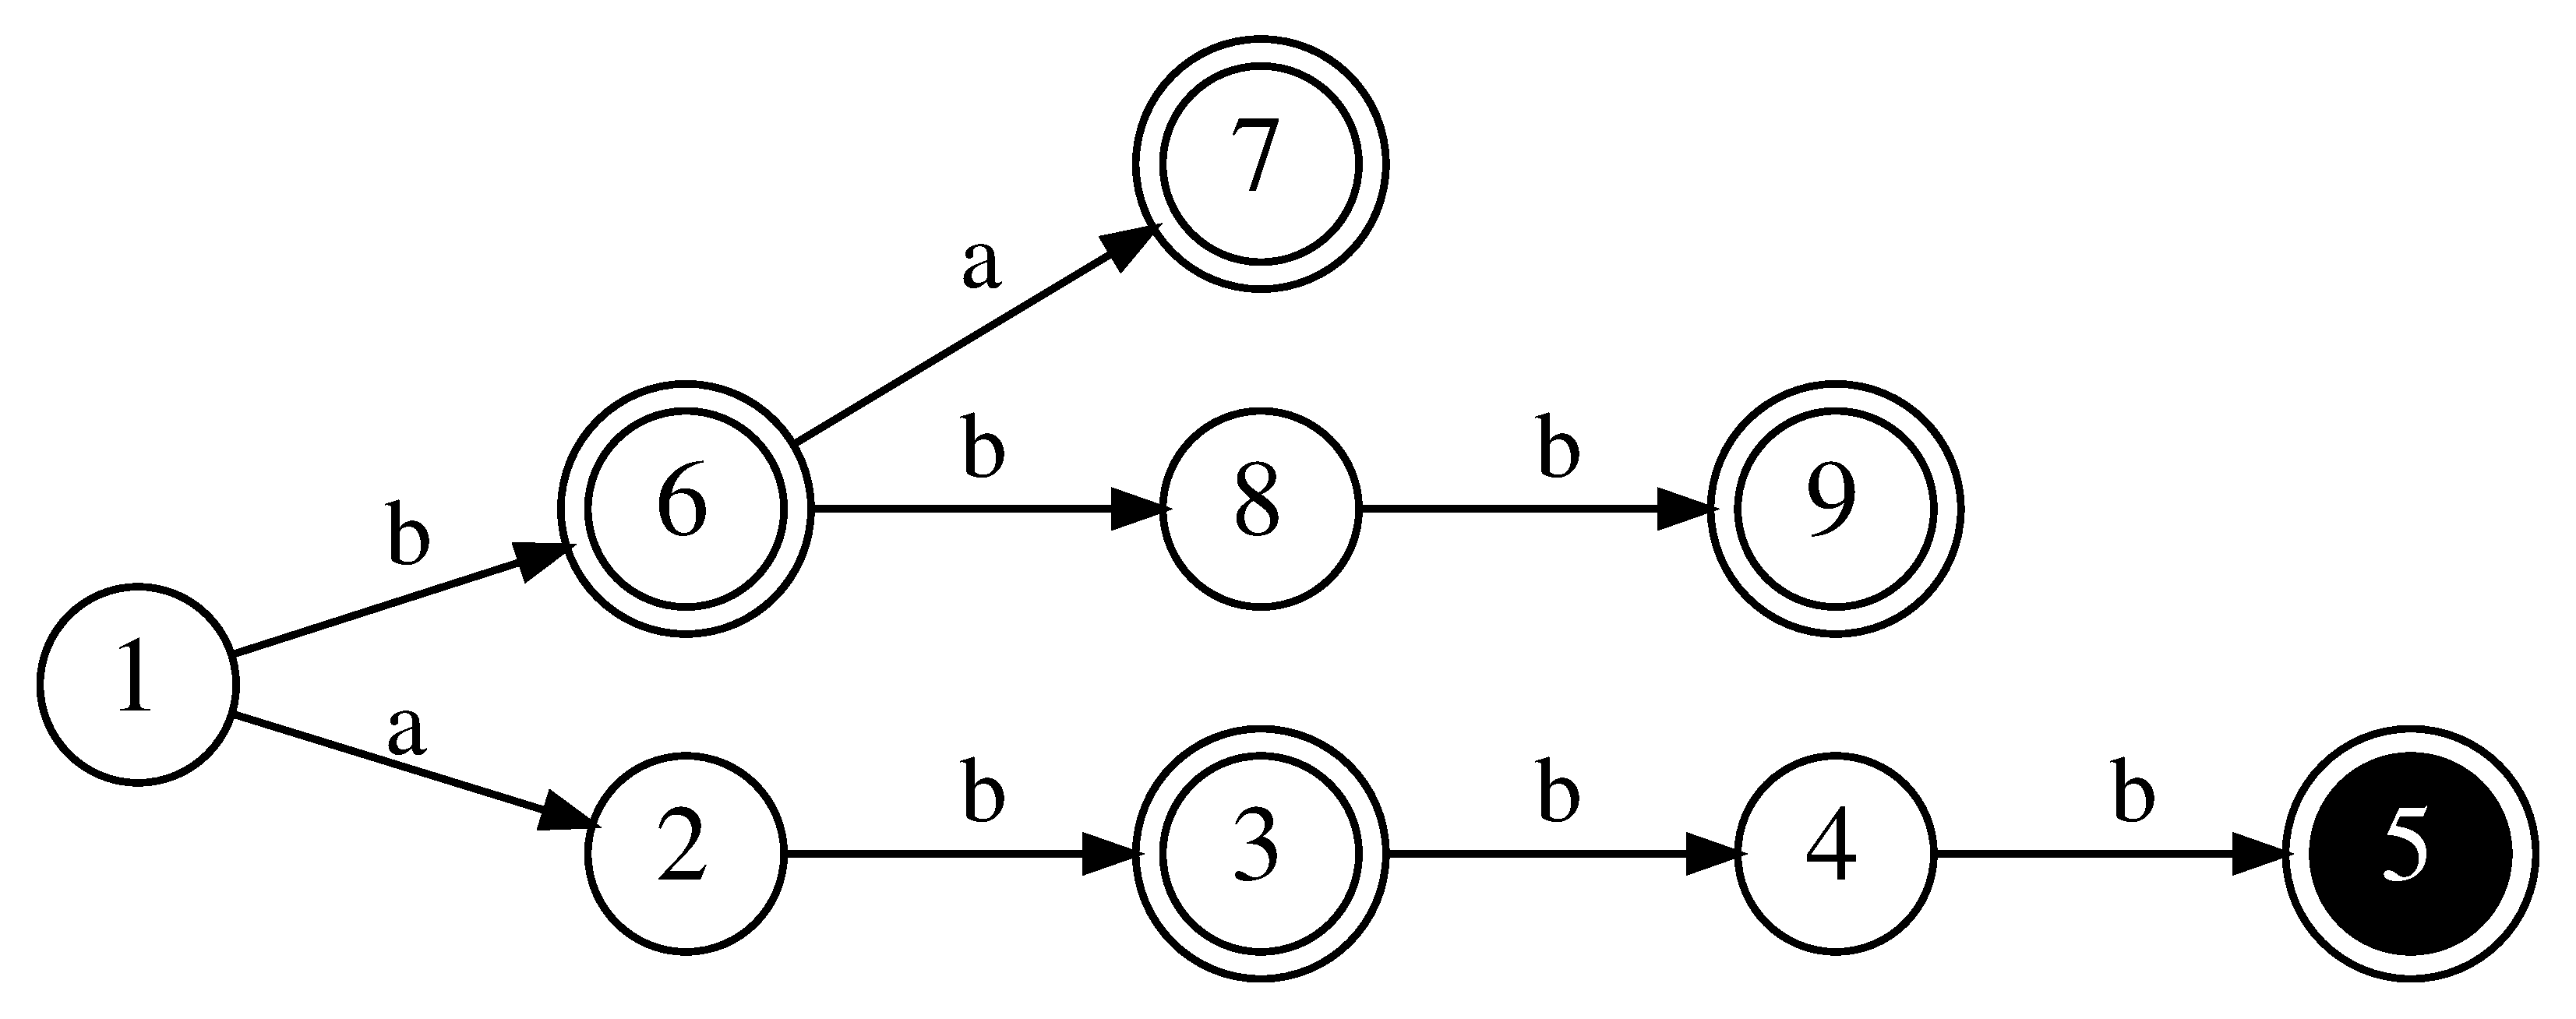
\includegraphics[scale=0.15]{img/datamod/FIG9a.eps}
  \caption{Пример расширенного префиксного дерева для множеств слов $S_{+}=\left\{ab,b,ba,bbb\right\}$ и $S_{-}=\left\{abbb\right\}$}
  \label{img:apta-loop}
\end{figure}
%
На рисунке~\ref{img:dfa-loop} представлен ДКА минимального размера, соответствующий расширенному префиксному дереву, изображенному на рисунку~\ref{img:apta-loop}.
Переход из состояния $2$ по символу $a$ в данном автомате не покрывается никакими переходами префиксного дерева, а значит является свободным.
С помощью предложенных ранее ограничений можно зафиксировать данный переход в виде петли, что продемонстрировано на рисунке штриховой линией.
%
\begin{figure}[ht]
  \centering
  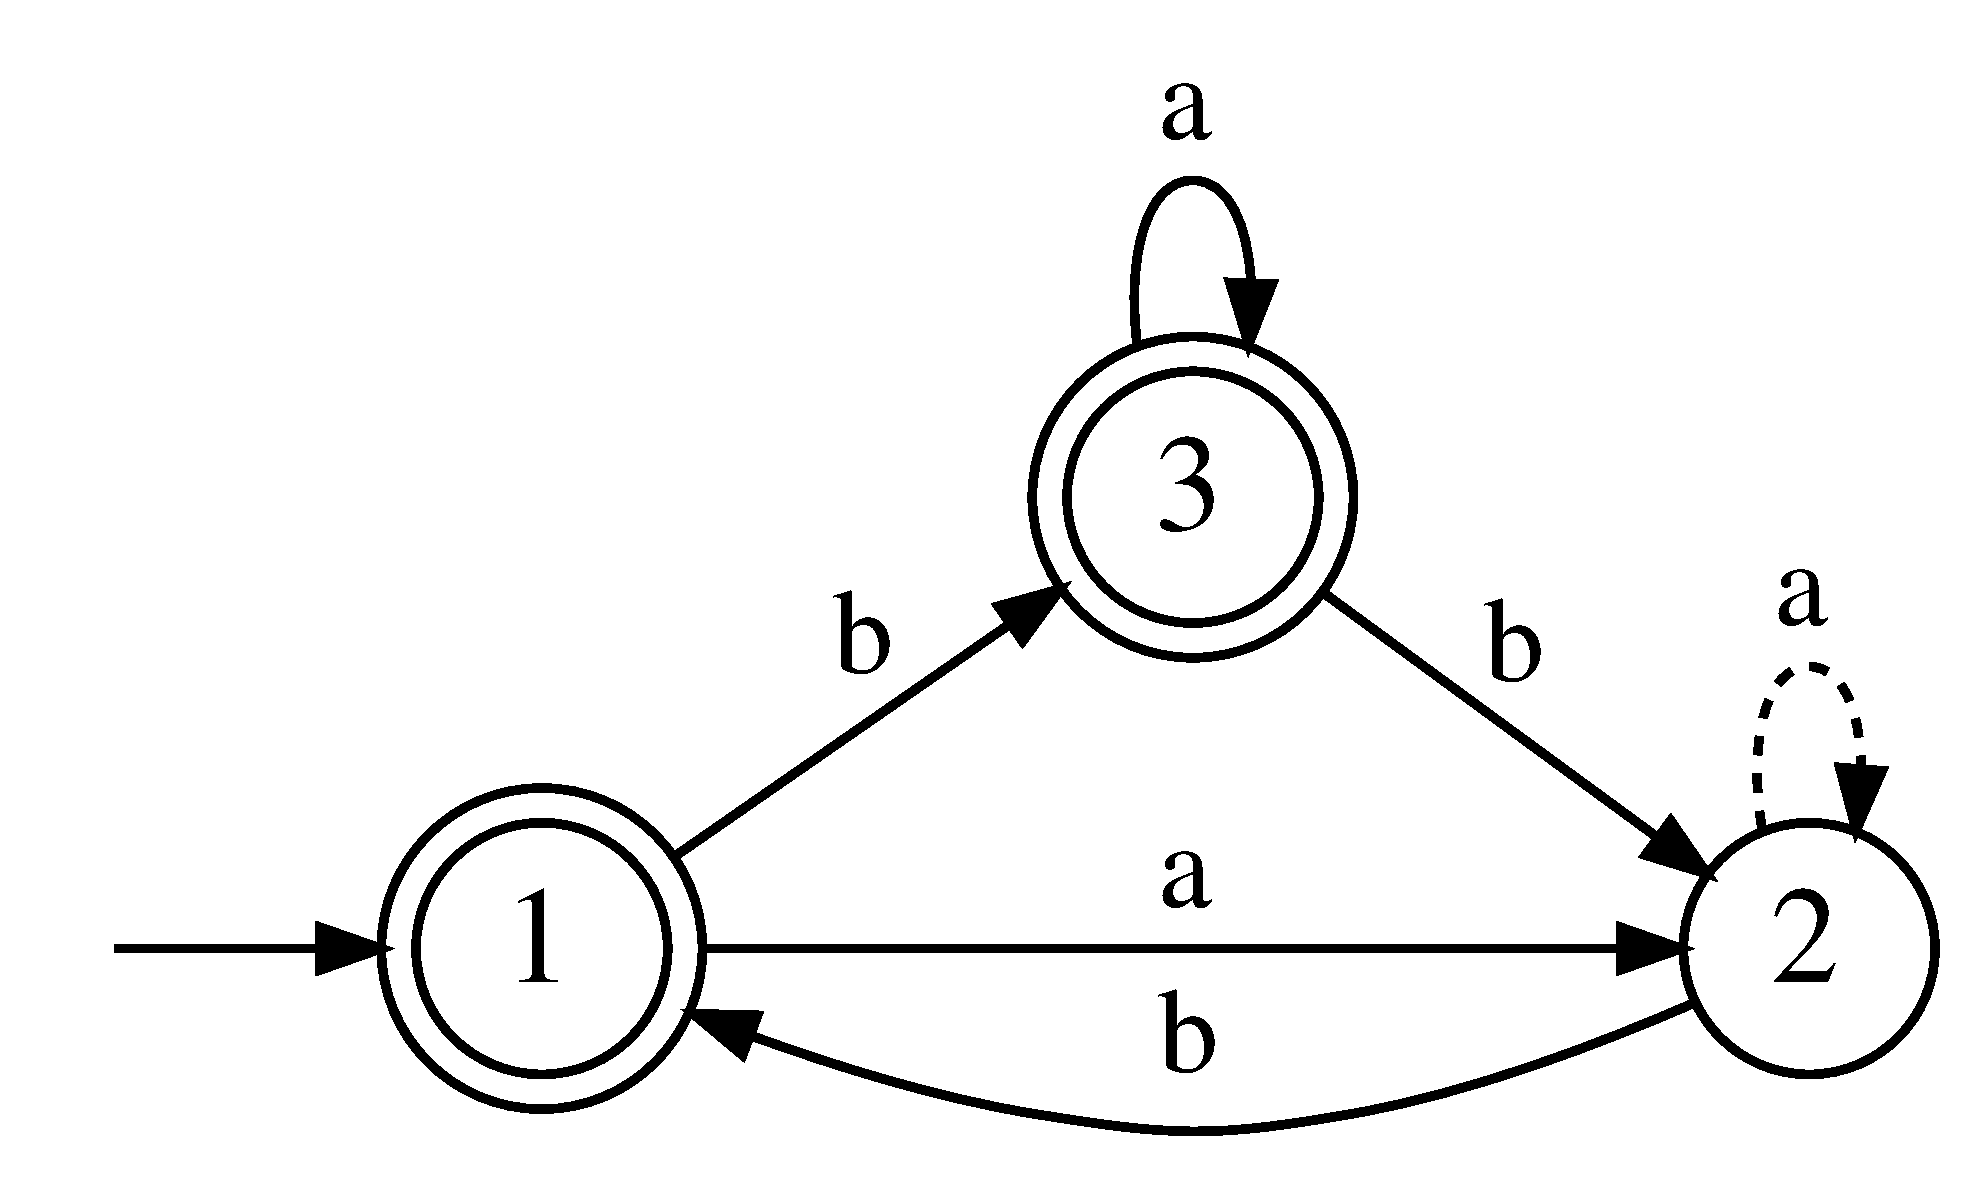
\includegraphics[scale=0.15]{img/datamod/FIG9b.eps}
  \caption{Пример ДКА, построенного по префиксному дереву, представленному на рисунке~\ref{img:apta-loop}, с зафиксированным свободным переходом из состояния $2$ по символу $a$}
  \label{img:dfa-loop}
\end{figure}

%----------------------------------------------------------------------------------------

\section{Реализация и экспериментальные исследования разработанных методов}
\label{sec:findall:results}

В настоящем разделе приводятся описание реализации разработанных методов и экспериментальные исследования, проведенные с ними.

%----------------------------------------------------------------------------------------

\subsection{Реализация разработанных методов генерации всех детерминированных конечных автоматов}
\label{sec:findall:results:impl}

Предложенный в предыдущем разделе метод генерации ДКА минимального размера на основе сведения к SAT и с использованием подхода уточнения абстракции по контрпримерам был реализован на языке \emph{python} как модуль программного комплекса \texttt{DFA-Inductor-py}.

%----------------------------------------------------------------------------------------

\subsection{Алгоритм перебора с возвратами}
\label{sec:findall:results:backtracking}

Так как ранее не предлагалось методов для поиска всех возможных примеров поведения по заданным словарям, то был разработан переборный алгоритм с возвратами, не использующий никаких сторонних программных средств.
Данный алгоритм работает следующим образом.
Изначально создается псевдоДКА $\mathcal{D}$ с $M$ вершинами (где $M$~--- размер искомого ДКА), но без переходов и без выделенных допускающих состояний, который затем будет достраиваться до полноценного ДКА.
Для этого на каждой итерации алгоритма поддерживается фронт расширенного префиксного дерева $\mathcal{A}$ $frontier$~--- множество ребер префиксного дерева $A$, для которых все предшествующие ребра на пути от корня дерева до них уже представлены в автомате $\mathcal{D}$, а они сами~--- еще нет.
Изначально фронт состоит из всех исходящих из корня дерева $\mathcal{A}$ ребер.
Рекурсивная функция $\mathtt{backtracking}$ поддерживает фронт в актуальном состоянии.
Если фронт не пуст, тогда данная функция пытается достроить текущий ДКА с помощью одного из ребер фронта.
После каждого достраивания текущий автомат проверяется на соответствие префиксному дереву, и, если противоречий не найдено, то фронт обновляется.
Если же фронт пуст, то все ребра префиксного дерева $\mathcal{A}$ представленны в автомате $\mathcal{D}$, а значит соответствующий автомат найден.
Тогда ДКА $\mathcal{D}$ проверяется на полноту, и, если автомат не полон, то недостающие переходы добавляются в виде петель (аналогично тому, как это предлагалось делать в предыдущем разделе с помощью переменных использования) с помощью функции $\mathtt{makeComplete}$.
Псевдокод разработанного метода представлен в листинге~\ref{algo:backtracking}.
Функция $\mathtt{findNewFrontier}$ возвращает новый фронт для дополненного ДКА или $\mathtt{NULL}$, если ДКА не соответствует расширенному префиксному дереву.
Данный алгоритм полного поиска основан на алгоритме из~\cite{DBLP:journals/sttt/UlyantsevBS18}.


\begin{algorithm}[ht]
  \caption{Переборный алгоритм с возвратами для генерации всех ДКА минимального размера}
  \label{algo:backtracking}
  \begin{algorithmic}[0]
    \Require расширенное префиксное дерево $\mathcal{A}$; %
    текущая версия искомого ДКА $\mathcal{D}$; %
    фронт $frontier$.
    \Ensure множество $S$ всех неизоморфных ДКА, соответствующих префиксному дереву $\mathcal{A}$.
    \\\hrulefill
    \Function{backtracking}{$\mathcal{A}, \mathcal{D}, frontier$}
      \State $S \gets \text{пустое множество}$
      \State $edge edge \gets \text{любое ребро из } frontier$
      \ForAll{$destination \in 1 \ldots \mathcal{D}.size$}
        \State $source \gets \text{состояние }\mathcal{D}\text{, которому соответствует } edge.from$
        \State $\mathcal{D'} \gets \mathcal{D} \cup \Call{transition}{source, destination, edge.label}$
        \State $frontier' \gets \Call{findNewFrontier}{\mathcal{A}, \mathcal{D'}, frontier}$
        \If{$frontier' \ne \mathtt{NULL}$}
          \If{$frontier' = \emptyset$}
            \State $S.add\left(\Call{makeComplete}{\mathcal{D'}}\right)$
          \Else
            \State $S.add\left(\Call{backtracking}{\mathcal{A}, \mathcal{D'}, frontier'}\right)$
          \EndIf
        \EndIf
      \EndFor
      \Return{$S$}
    \EndFunction
  \end{algorithmic}
\end{algorithm}

%----------------------------------------------------------------------------------------

\subsection{Экспериментальные исследования разработанных методов генерации всех детерминированных конечных автоматов}
\label{sec:findall:results:dfs}

Все эксперименты проводились на сервере с 64-ядерным процессором \texttt{AMD Opteron 6378 @ 2.4 ГГц} и операционной системой \texttt{Ubuntu 14.04}.
Для генерации тестовых данных снова использовался алгоритм, предложенный в разделе~\ref{sec:space:results:random-input}.
Использовались следующие параметры: размер искомого автомата $M \in \left[5; 15\right]$, мощность алфавита $L = 2$, суммарное число примеров поведения $S \in \left\{5 \times M; 10 \times M; 25 \times M\right\}$.
Для каждого набора параметров генерировалось по 100 различных автоматов и соответствующих наборов примеров поведения.

Сравнивались три метода генерации всех неизоморфных ДКА по примерам поведения:
\begin{itemize}
  \item метод, основанный на сведении к SAT, из раздела~\ref{sec:findall:SAT-based} с перезапуском программного средства для решения SAT (столбец REST в таблице);
  \item метод, основанный на сведении к SAT, из раздела~\ref{sec:findall:SAT-based} с использованием инкрементального программного средства для решения SAT (INC);
  \item переборный метод с возвратами из раздела~\ref{sec:findall:backtracking} (BTR).
\end{itemize}
Результаты экспериментальных исследований представлены в таблице~\ref{tab:find-all}.
Ограничение по времени было установлено в один час (3600 секунд).
Столбец $>$1 показывает процент экземпляров задачи, где существовало больше одного неизоморфного автомата.
Так как в таблице представленно медианное время, то если менее 50 (то есть менее половины) экземпляров были решены, то в соответствующей ячейке стоит прочерк (---).

\begin{table}[ht]
  \centering
  \caption{Медианное время нахождения всех различных ДКА с помощью метода на основе сведения к SAT с перезапуском программного средства (REST), метода на основе сведения к SAT с использованием инкрементального программного средства (INC) и переборного метода с возвратами (BTR)}
  \scalebox{0.65}{
    \begin{tabular}{ccccccccccccccc}
      \hline
      \multirow{2}{*}{$M$} & \multicolumn{4}{c}{$S = 5 \times M$}  & ~ & \multicolumn{4}{c}{$S = 10 \times M$} & ~ & \multicolumn{4}{c}{$S = 25 \times M$}\\\cline{2-5}\cline{7-10}\cline{12-15}
         & $>$1& REST &  INC    & BTR            & & $>$1& REST  & INC  & BTR             & & $>$1& REST & INC  & BTR            \\\hline
      5  & 53  & 2.3   & 2.0   & 0.8            & & 40  & 3.6   & 3.3  & 1.3             & & 17  & 4.1  & 3.4  & 1.5           \\ 
      6  & 56  & 2.8   & 2.4   & 2.1            & & 31  & 4.7   & 3.9  & 1.7             & & 27  & 5.4  & 4.3  & 1.7           \\ 
      7  & 87  & 3.9   & 2.5   & 4.1            & & 27  & 3.7   & 3.0  & 3.1             & & 13  & 7.4  & 6.7  & 2.5          \\ 
      8  & 80  & 4.6   & 3.7   & 87.2           & & 34  & 7.0   & 6.5  & 41.7            & & 16  & 10.1  & 8.9 & 11.6 \\ 
      9  & 91  & 7.6   & 3.9   & 475.1          & & 50  & 7.7   & 6.4  & 121.6           & & 10  & 13.8 & 13.0 & 61.4 \\ 
      10 & 89  & 15.7  & 5.3   & 2756.2         & & 47  & 8.6   & 7.0  & 974.7           & & 11  & 18.8 & 16.1 & 276.8 \\
      11 & 94  & 19.9  & 7.3   & ---             & & 63  & 18.5  & 13.8 & 3108.0          & & 9   & 24.5 & 21.9 & 1158.4 \\
      12 & 90  & 28.0  & 9.9   & ---             & & 49  & 22.3  & 16.7 & ---              & & 8   & 33.5 & 27.2 & 3289.1 \\
      13 & 92  & 185.5 & 18.1  & ---             & & 57  & 36.9  & 22.6 & ---              & & 12  & 62.0 & 51.4 & --- \\
      14 & 87  & 408.5 & 49.0  & ---             & & 71  & 85.1  & 41.8 & ---              & & 4   & 67.0 & 56.2 & --- \\
      15 & 95  & 571.1 & 174.1 & ---             & & 69  & 193.3 & 95.7 & ---              & & 6   & 29.2 & 26.2 & --- \\
      \hline
    \end{tabular}
  }
  \label{tab:find-all}
\end{table}

Результаты экспериментов позволяют сделать несколько выводов.
Во-первых, впервые успешно решена задача генерации всех различных ДКА минимального размера по заданным примерам поведения.
Во-вторых, оба метода, использующие сведение к SAT, значительно превосходят по производительности переборный метод.
В-третьих, использование инкрементального программного средства, как и предполагалось, дает заметное преимущество относительно подхода с перезапуском программного средства, что объясняется сохранением промежуточного состояния инкрементальным программным средством после нахождения некоторого ДКА.
В-четвертых, чем больше примеров поведения дано для генерации ДКА, тем реже случается ситуация, когда существует несколько различных ДКА, соответствующих им.
Однако, надо заметить, что помимо количества примеров поведения, их качество не менее важно.


%----------------------------------------------------------------------------------------

\chresults{\ref{sec:findall}}

% %!TEX root = ../dissertation.tex

\chapter*{Заключение}                       % Заголовок
\addcontentsline{toc}{chapter}{Заключение}  % Добавляем его в оглавление

%% Согласно ГОСТ Р 7.0.11-2011:
%% 5.3.3 В заключении диссертации излагают итоги выполненного исследования, рекомендации, перспективы дальнейшей разработки темы.
%% 9.2.3 В заключении автореферата диссертации излагают итоги данного исследования, рекомендации и перспективы дальнейшей разработки темы.
%% Поэтому имеет смысл сделать эту часть общей и загрузить из одного файла в автореферат и в диссертацию:

Основные результаты работы заключаются в следующем.
%!TEX root = ../dissertation.tex
\begin{enumerate}
  \item .
  \item .
  
\end{enumerate}

...

      % Заключение

\clearpage\urlstyle{rm}\printbibliography\urlstyle{tt}
% \clearpage\listoffigures
% \clearpage\listoftables
\newpage

%%% Настройки для приложений
% \appendix
% \counterwithin{figure}{chapter}
% \counterwithin{table}{chapter}
%\counterwithin{algorithm}{chapter}
%\counterwithin{lstlisting}{chapter}
\renewcommand{\thechapter}{\Asbukx{chapter}}

% %!TEX root = ../dissertation.tex

...        % Приложения

% \clearpage
% \chapter*{Публикации} \addcontentsline{toc}{chapter}{Публикации}
% 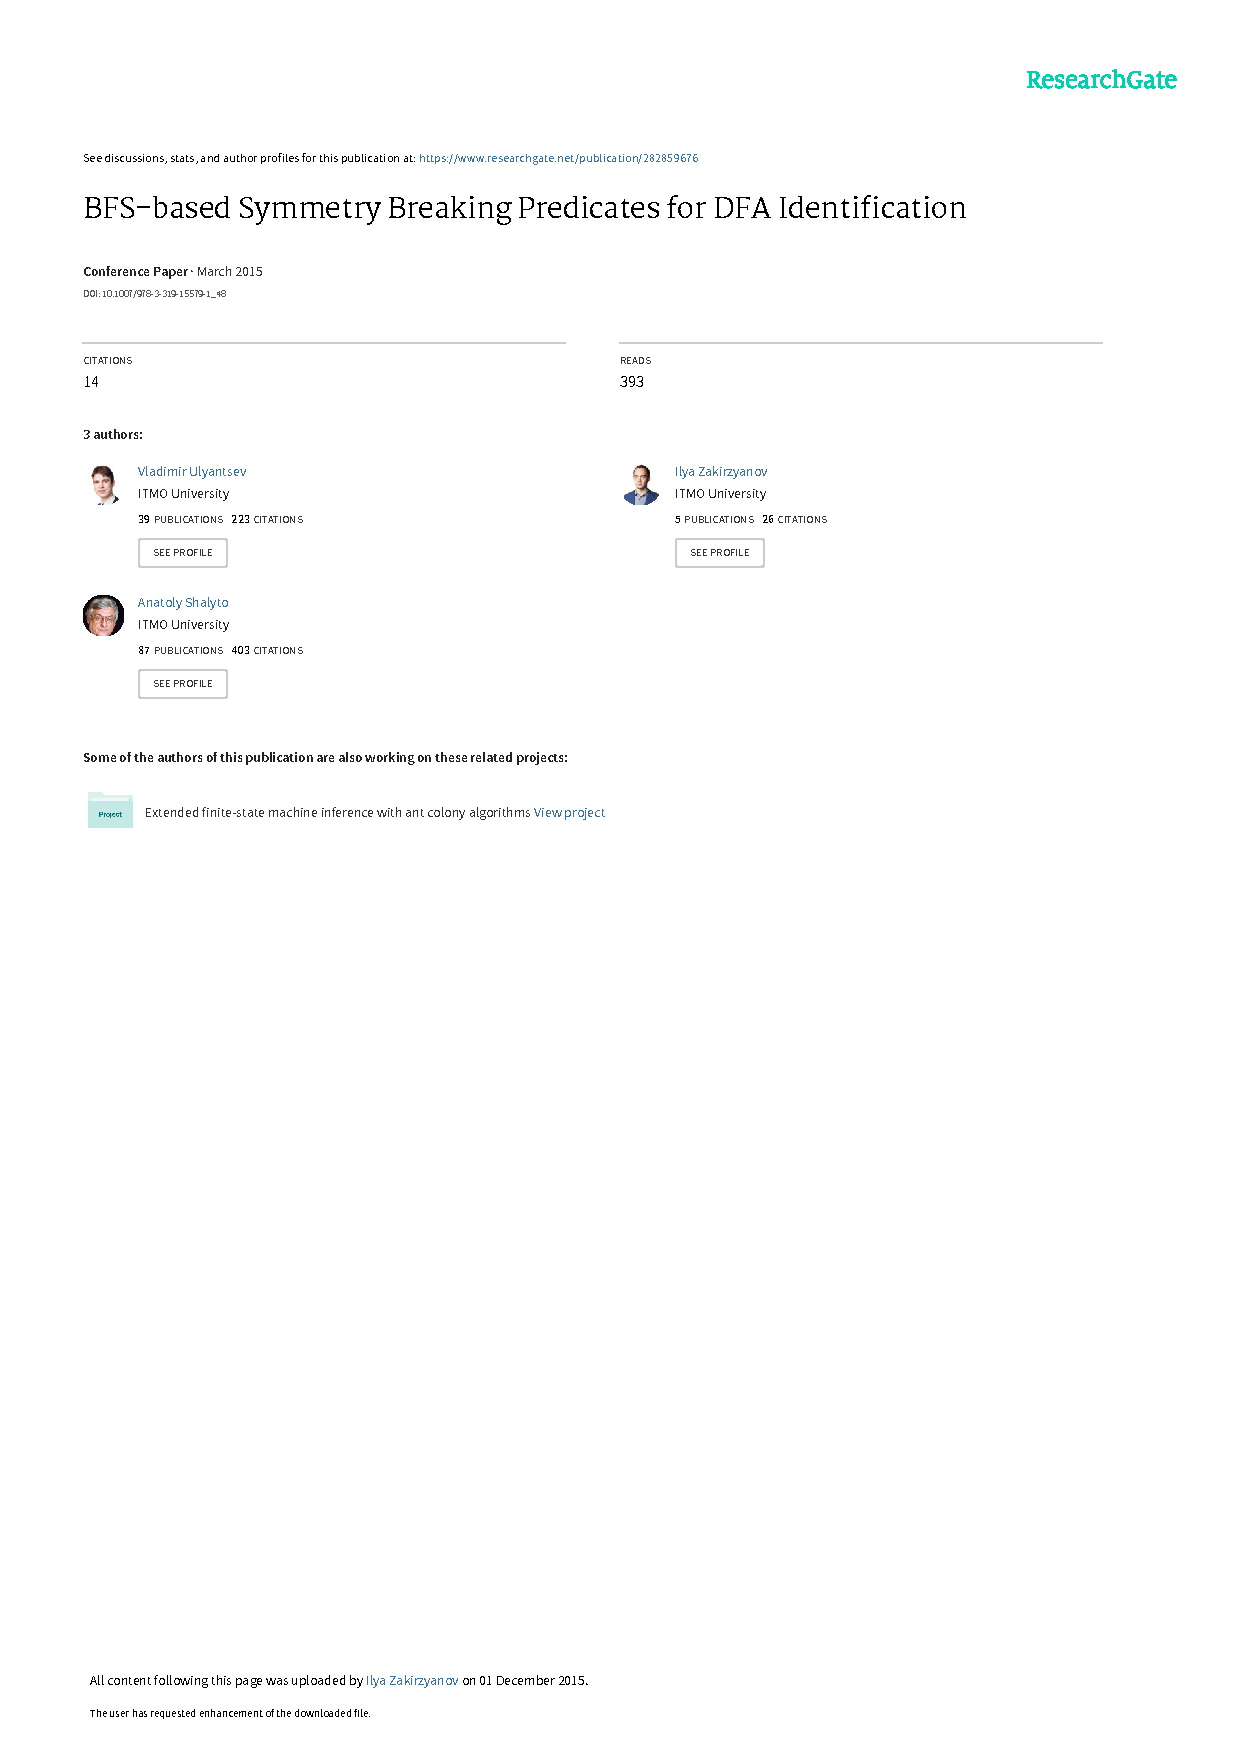
\includepdf[pages=-]{Papers/2015-LATA.pdf}
% 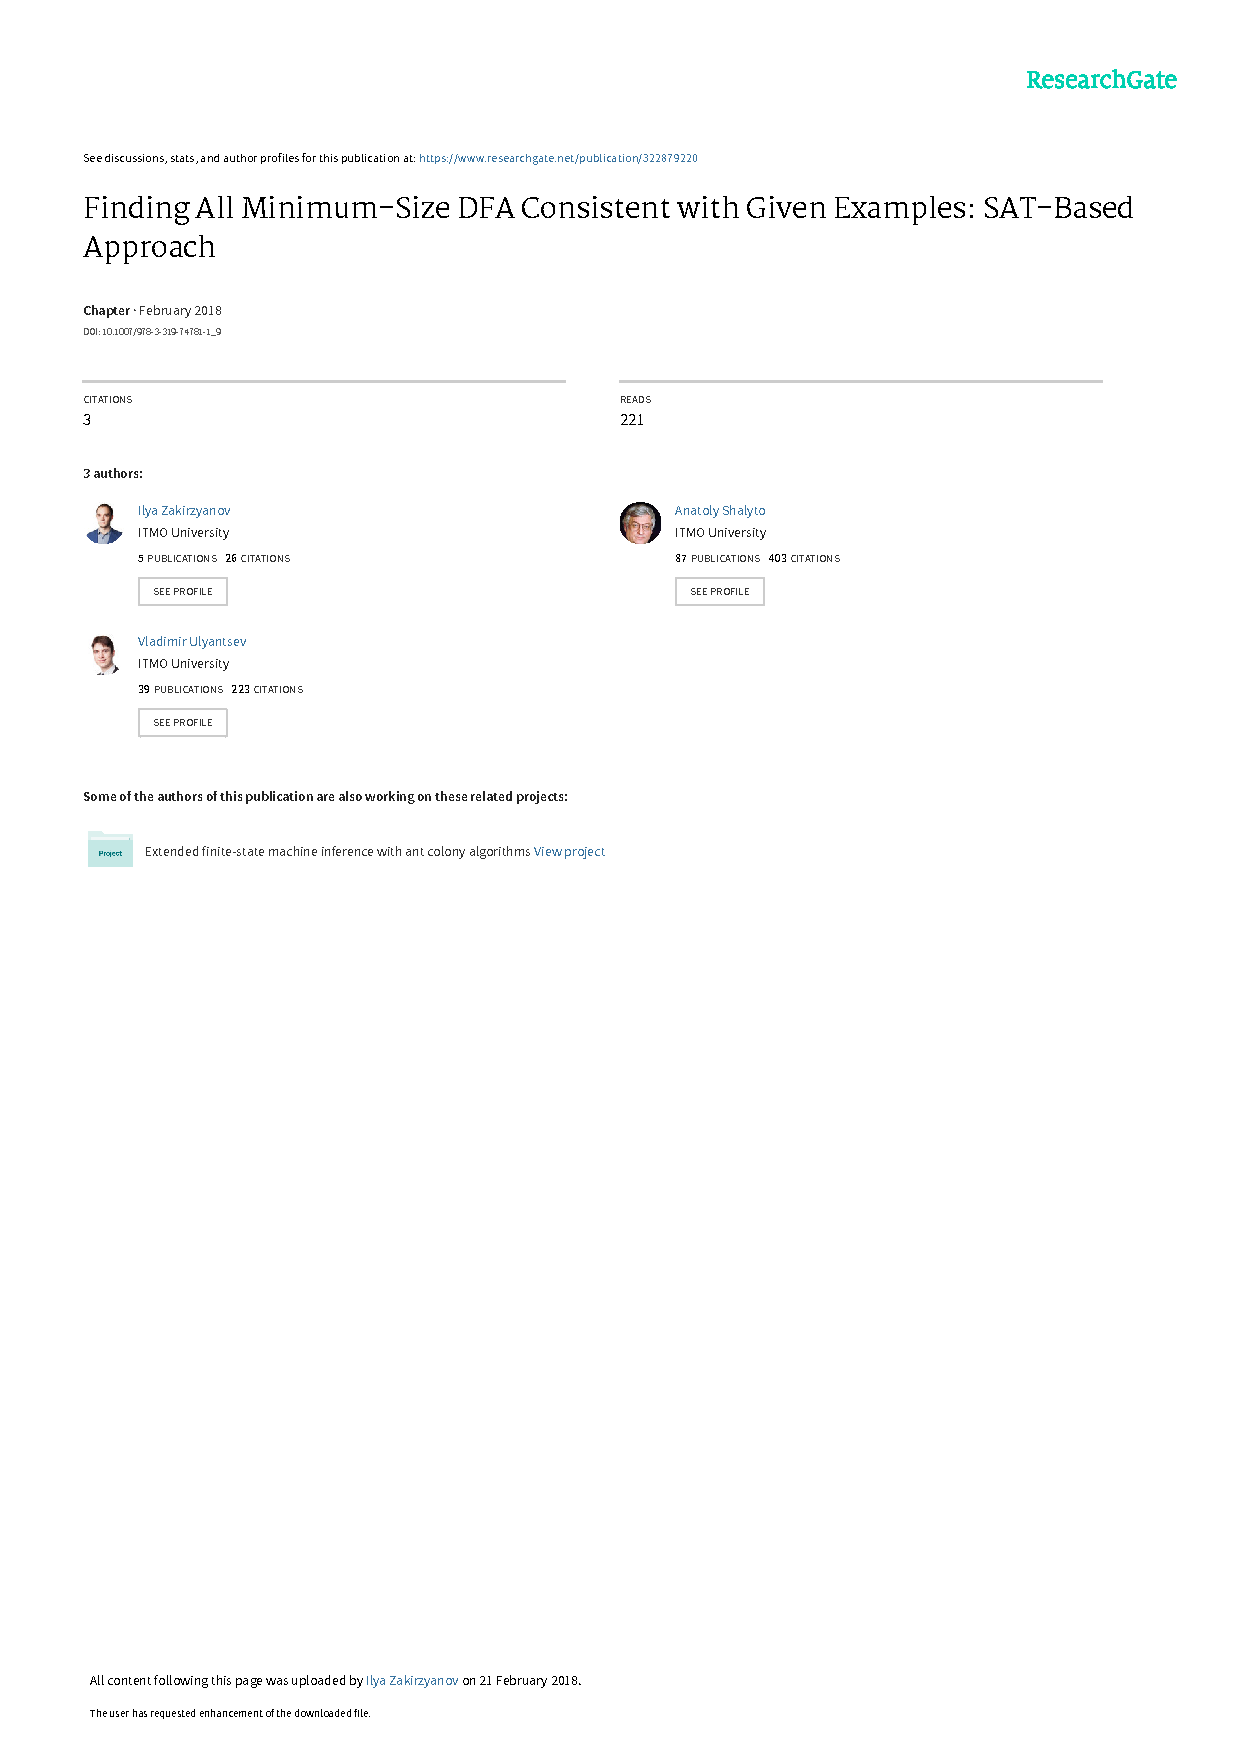
\includepdf[pages=-]{Papers/2017-DataMod.pdf}
% 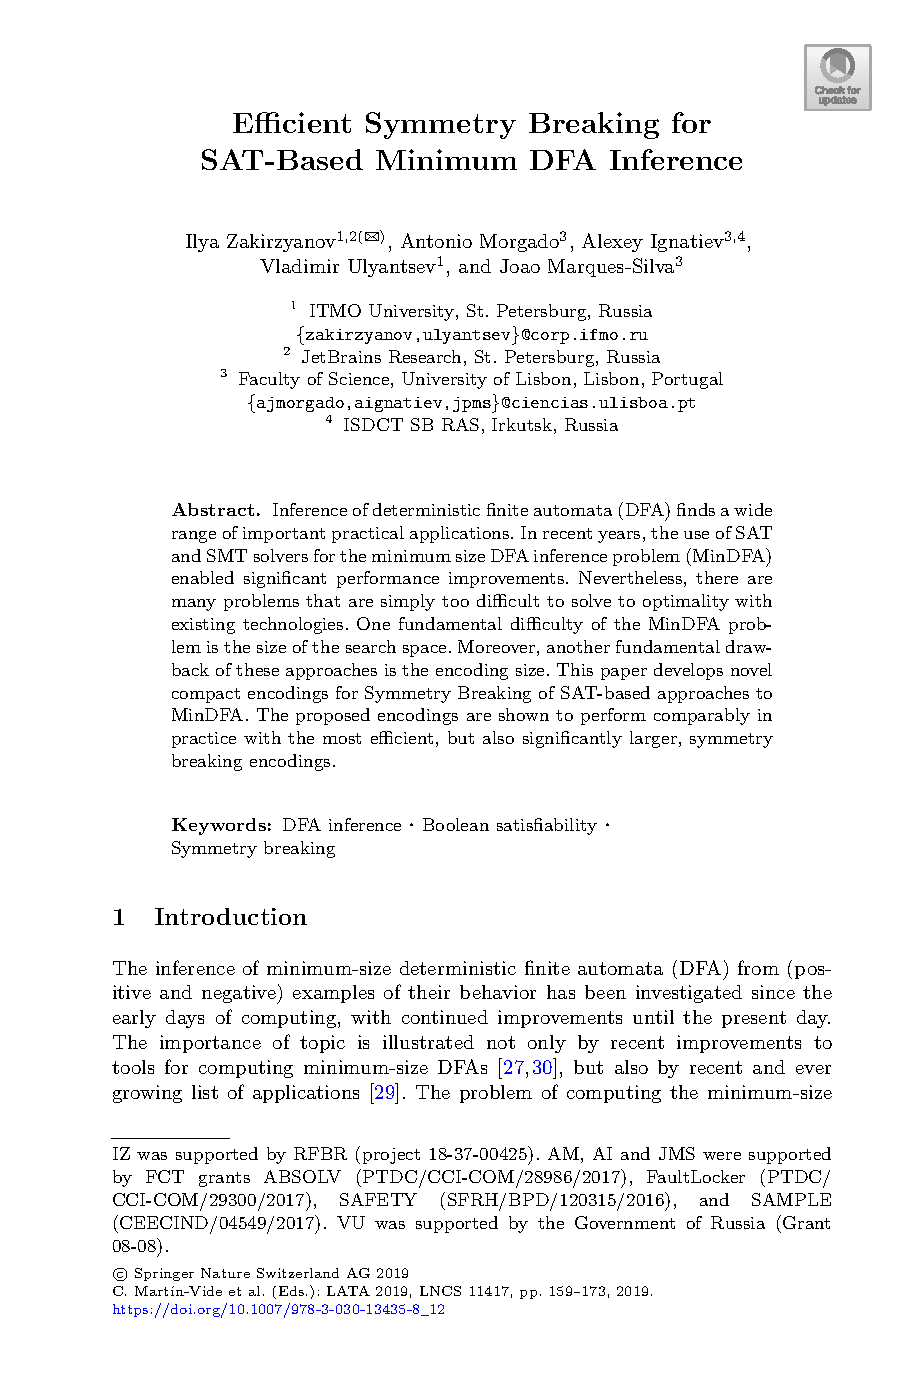
\includepdf[pages=-]{Papers/2019-LATA.pdf}
% 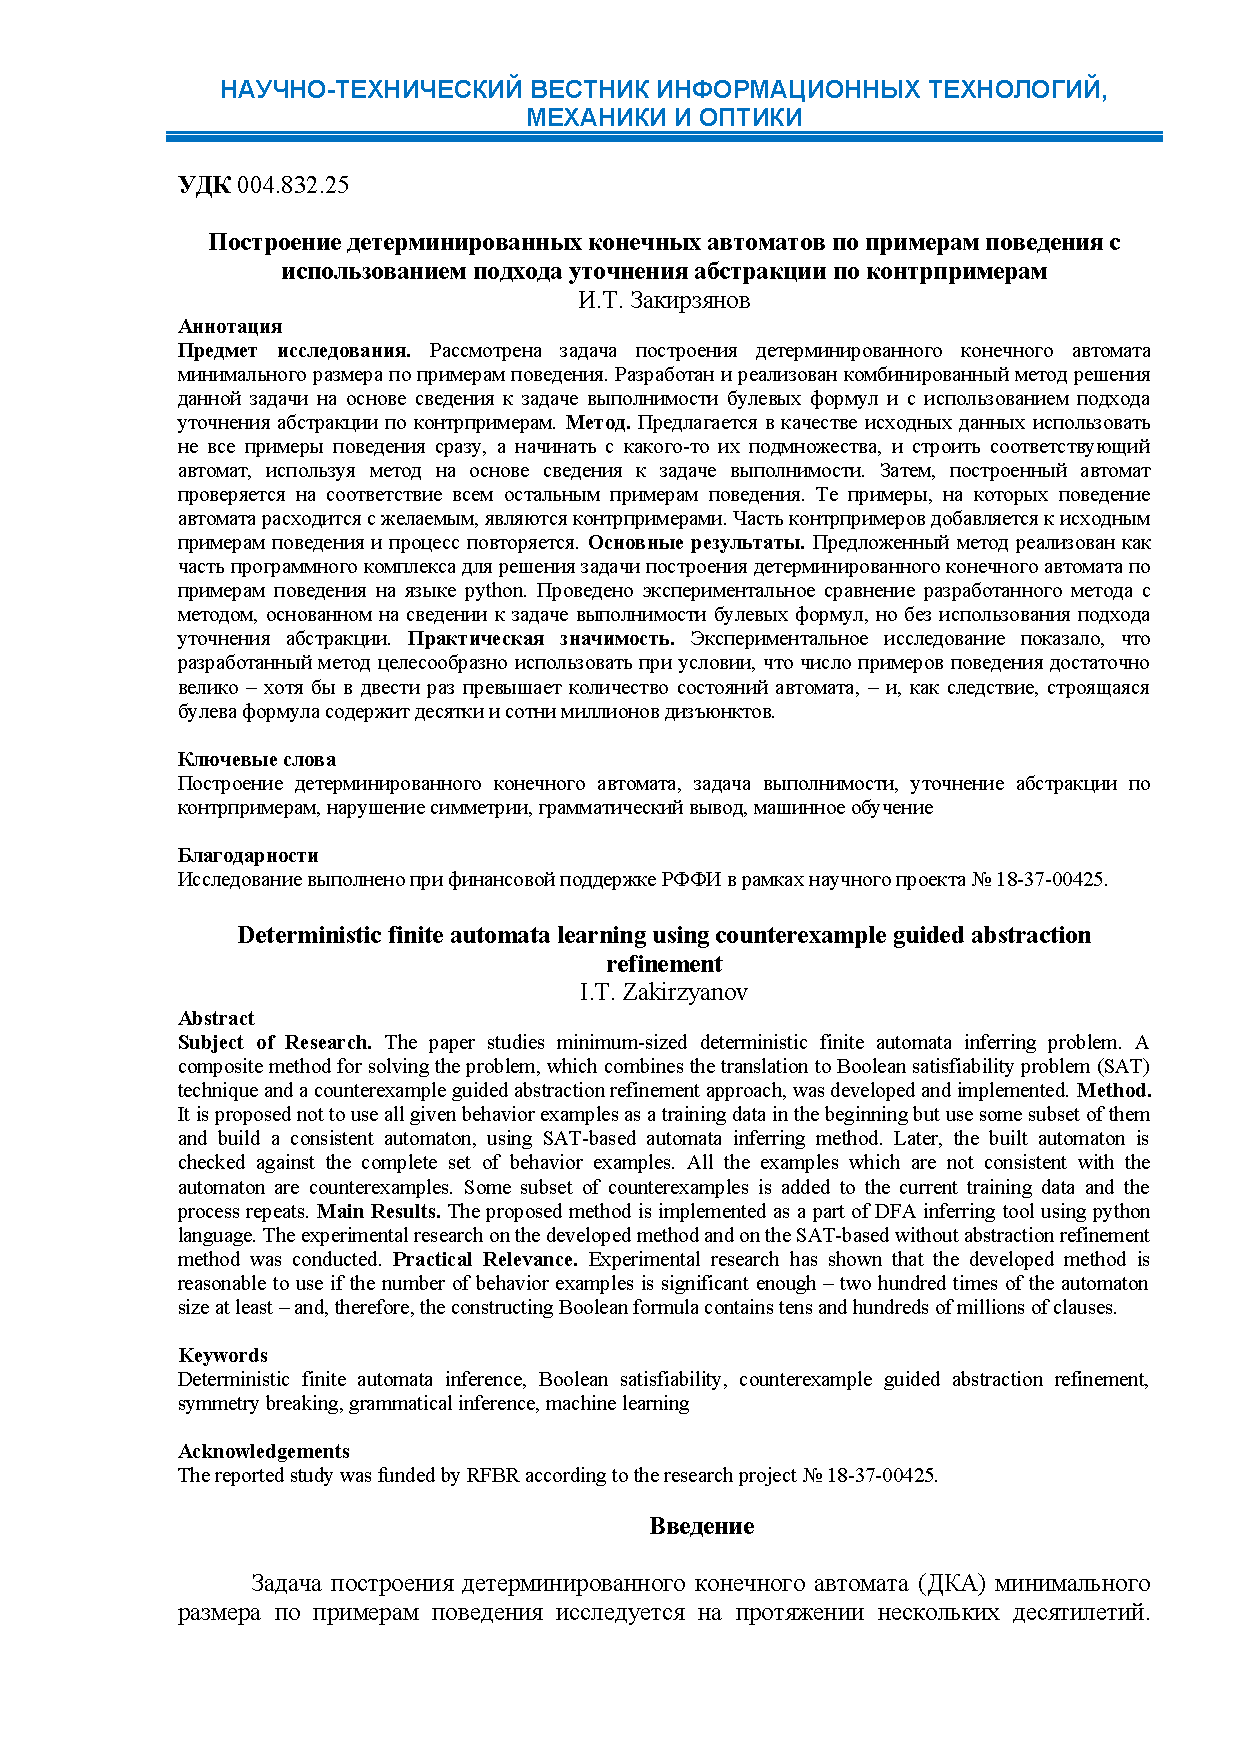
\includepdf[pages=-]{Papers/2020-Vestnik.pdf}

\end{document}
